\section{ALL PLACHOLDER SECTIONS COME HERE}

\section{Dataset Description}
\label{sec:dataset}

In this section, we describe the three datasets: \moball, \mobcomp, and \mobexpt. 
We use these datasets in our studies that we present in the subsequent sections.

\tbd{Run genDataSetDescription.R to get these numbers} 
The \moball dataset consists of mobile data traffic traces from \tbdv{23} devices that belong to \tbdv{18} users who are volunteers of an IRB approved study. 
This dataset consists of \tbdv{8} iPhones, \tbdv{3} iPads, \tbdv{1} iPodTouch, \tbdv{10} of Android phones, and \tbdv{1} of Android tablet.
We consider an Android device that accesses the Internet by using only \wifi to be a tablet. 
The Android devices used to generate this dataset include the Nexus, Sony, Samsung, and Gsmart brands. 
The users of these devices are spread across France and USA. We observed connections from \tbdv{52} different ISPs.
This dataset consists of \tbdv{171} days of data that was captured on our servers and for each device the number days varies from \tbdv{5} to \tbdv{171} with a median of \tbdv{34} days.  

The \mobcomp dataset consists of data from two users who had three and two devices respectively. 
The three devices that belong to one of the two users consists of a two smart phones and a tablet, while one smartphone and a tablet belong to the second user. 
We use this dataset to compare the behavior of popular apps and to detail the behavior of devices when the device is kept idle. 
The data set consists of \tbdv{number} of days of data from each device and \tbd{number} of days for which data traffic was seen for all the 24 hours. 

The \mobexpt dataset contains the traffic traces from an Android device and an iOS device that were used to perform a controlled experiment on popular application. 
We tested \tbdv{number} of Android applications and \tbdv{number} of iOS application for this study. 
\tbd{How we decided this list}. \tbd{How we performed the test} \tbd{other attributes of this dataset}.

%%% Local Variables: 
%%% mode: latex
%%% TeX-master: "main"
%%% End: 


%\section{Evaluation}
\label{sec:eval}
This section evaluates \meddle in terms of overhead, visibility into network traffic and 
the ability to map network traffic to the apps that generated it. We use the results in 
this section to inform the applications we build in \S\ref{sec:characterize-app} and \S\ref{sec:isp-behavior}.

\subsection{Methodology}
\label{sec:dataset}
Using \platname, we collected full packet traces from Internet activity generated by
mobile devices. We use this data to study how to map monitored traffic to applications, and to
analyze PII leakage. Below, we describe our data-collection methodology, which consists of
1) controlled experiments in a lab setting and 2) IRB-approved ``in the wild'' measurements 
gathered from real users during seven months.


\subsubsection{Controlled Experiments with Apps}
\label{sec:dataset-contr-exper}
Our goal with controlled experiments is 1) to obtain ground truth information 
about network flows generated by apps and devices, and 2) characterize the 
network activity for a large variety of apps in a lab setting. We use 
this data to understand how to model apps' network behavior, how to map network flows 
to the app that generated them and how to identify PII in those network flows. 

\noindent\textbf{Device setup.} We conducted our controlled experiments using two Android 
devices (running Android 4.0 and 4.2) and an iPhone running iOS 6. We start each set of controlled experiments
 with a factory reset of the device to ensure that software installed by previous 
 experiments cannot impact the network traffic generated by each device. 
 Then we connect the device to \platname{}  and begin
the experiment. 


\noindent\textbf{SSL bumping.} 
We use SSL bumping only in controlled experiments where \emph{no user traffic is intercepted}.
%, using a plugin to enable % SSL traffic decryption. 
We are also designing a study for IRB approval in which users can opt in to use SSL bumping for obfuscating PIIs in their SSL traffic.

\noindent\textbf{Manual tests.} We manually test the
100 most popular free Android apps in the \emph{Google Play} store and 209
iOS apps from the iOS App store on April 4, 2013. For each
app, we install it, enter user credentials %for the account 
if relevant, interact with it for up to 10 minutes, and uninstall
it. This allows us to characterize real user interactions with popular apps
in a controlled environment.  
We enter unique and distinguishable user credentials when 
interacting with apps to easily extract the corresponding PII from 
network flows (if they are not obfuscated). We use the same technique 
to test malware apps (\S\ref{subsec:malware}).

\noindent\textbf{Automated tests.} The second set of controlled experiments consist of fully-automated
experiments on 732 Android apps from a free,
third-party Android market, \emph{AppsApk.com}~\cite{appsapk}.
We perform this test because Android users can install
\emph{Third-party apps} without rooting their device. 
% that are not available on the
%\emph{Google Play} store, 

Our goal is to understand how these apps differ from those in the standard \emph{Google Play} 
store, as they are not subject to Google Play restrictions.
%\tbd{Is there different constraints on this free market, AR: They do not have paid application. All apps must be free.}
We automate experiments using \emph{adb} to
install each app, connect the device to the \meddle platform, and
start the app. Then we use \emph{Monkey}~\cite{adbmonkey}, an app-scripting 
tool, to perform a series of  approximately 100,000 actions that include
random swipes, touches, and text entries.  Finally, we use adb to
uninstall the app and reboot the device to forcibly end any
lingering connections. This set of experiments is limited to
Android devices because iOS does not provide equivalent 
scripting functionality. 
%\tbd{Are they stores from which you can download apps for non jail-broken iOS devices? DC: No.}

\subsubsection{In Situ Study}
\label{sec:dataset-wild-measurements}

The controlled experiments in the previous section provide us with 
ground-truth information for a large number of apps running in a controlled 
setting for a short period of time. To understand the network behavior of 
devices with real users ``in the wild'' over longer time periods, we conducted 
an IRB-approved measurement study with a small set of subjects, from 
Oct. 15, 2012 to Sep. 1, 2013.\footnote{The measurement study is ongoing, we report a subset of results.}

Our measurement data was collected from 26 devices: 10 iPhones, 4 iPads, 1 iPodTouch, and 11
Android phones.  The Android devices in this dataset include the
Nexus, Sony, Samsung, and Gsmart brands while the iPhone devices
include one iPhone~3GS, four iPhone~5, and five iPhone~4S.  These
devices belongs to 21 different users, volunteers for our IRB approved
study.  This dataset, called \mobWild, consists of 318 days with data; the number of 
days for each user varies from 5 to 315 with a median of 35 days.  For privacy reasons, the
SSL-Bumping plugin is \emph{disabled} for all measurements involving
real users.


\subsection{Overheads}
\noindent\emph{Network Latency.}
We first test indirection overhead from mobile networks to a \meddle instance. In the 
US with EC2, delays from mobile-network egress points to EC2 nodes are on generally less than 10\,ms. 
For other networks, we will achieve similarly low indirection overhead by placing instances in a cloud/hosting 
provider near subscribers and use DNS redirection (\eg via Amazon's Route 53) to direct clients to nearby instances. 

The other source of network delays is connection establishment time, incurred once per session. We measured 
50 VPN-connection establishment times on both iOS (iPhone 5 / iOS 6.1) and Android (Galaxy Nexus /
Android 4.2), for \wifi{} and cellular connections. We conduct tests in rapid succession to ensure the radio is in the high power state.
The \meddle server was running on a university network. 
For Android (using IKEv2), the maximum establishment time was 0.81 seconds on \wifi{} and 1.59 seconds on cellular. 
For iOS (using IKEv1), the connection takes longer due to the older protocol version: we observe a maximum of 2 seconds on \wifi{} and 2.18 seconds on cellular. 
Because each VPN session supports many flows, the amortized cost of connecting is  small. 
%\tbd{Cite results from latency to home gateways based on DSL results in PAM and IMC.}
%\tbd{Address comments in conext review on latency}

\noindent\emph{Power Consumption.}
Mobile devices expend additional power to establish, maintain and encrypt data for a VPN tunnel. 
To evaluate the impact on battery, we used a power meter to measure the draw from a Galaxy Nexus running Android 4.2. 
We run 10-minute experiments with and without the VPN enabled. 
For each experiment, we used an activity script that included Web and map searches, Facebook interaction, e-mail and video
streaming. 
The VPN leads to a 10\% power overhead. 
For iOS devices, we relied on the battery readings provided by iOS because we cannot attach a power meter directly to the battery.
We again found an approximately 10\% power overhead of using VPNs when we drained a fully charged battery while performing the operations performed during the tests for Android devices.  

%\item 
\noindent\emph{Traffic Volume.}
\meddle relies on IPsec for datagram encryption, thus there is an encapsulation overhead for each tunneled packet. 
To evaluate this overhead, we use 30 days of data from 25 devices that to compare encapsulated and raw packet sizes. 
We observe a maximum encapsulation overhead of 12.8\% (average approximately 10\%). 
For users that have limited data plans and consume most of their quota per month, this can have 
a significant impact. We note that this is partially offset by \meddle services such as content filtering and 
connection blocking. % and optimizations such as transcoding and compression. 

\noindent\emph{Scalability.} We currently use Amazon EC2 to support users at our cost. 
Without exploring opportunities for economies of scale, we estimate that 
it will cost less than a penny (\$0.0084) per user per day. At this cost, we can support up to 
10,000 users with research funds. If \meddle were to become extraordinarily popular, it would 
cost each user approximately a quarter per month to pay their own way. By comparison, 
data plans in the US tend to cost \$30-\$90 per month -- more than two orders of magnitude larger.

\subsection{Meddle Visiblity}

%We now highlight key features of the \mobWild dataset. 
We now use data gathered from users to demonstrate that there is a need for a platform like \meddle that provides a comprehensive view of Internet traffic from mobile devices. 
Note that due to the relatively small number of users in our study, we do not attempt to  
draw strong and generalizable conclusions. 

\noindent\textbf{Observation 1: \emph{End-host instrumentation provides a more complete view of 
Internet traffic from mobile devices.}} We infer the access technology (WiFi or cellular) for 
each session with the AS description from a \emph{WHOIS} lookup for each IP address used by a mobile device.
Based on this classification, the \mobWild dataset consists of traffic from 65 distinct ASes, of which 8 are cellular ASes and 7 are university networks.

We observe less diversity in cellular ASes compared to \wifi ASes.
During the measurement study, each device connected to our \platname server from at most two distinct cellular ASes. 
In contrast, a median of 4 \wifi ASes were observed per device and for one device we observed traffic from 36 different \wifi ASes spread across 5 countries.
In terms of traffic volumes, collectively our users with cellular connectivity transferred 24-56\% of their traffic over cellular and the remainder over WiFi. 
The key take-away is that, for the users in the \mobWild dataset, we would miss a large fraction of traffic generated by the mobile devices by instrumenting a single cellular carrier or WiFi access point. 
\meddle does not have this limitation.

\noindent\textbf{Observation 2: \emph{\meddle provides visibility into a wide range of traffic patterns}.} 
We use the classification provided by Bro~\cite{bro} to categorize flows as either TCP, UDP, or \emph{other}, along with subcategories HTTP, SSL and DNS.
Table~\ref{tab:summaryIOSAndroidTraffic} summarizes the traffic generated by user devices in our study. 

There are three key take-aways from this table. 
First, Web and SSL traffic dominate the traffic for users in the \mobWild dataset; 91.26\% (137.63 GB) of the traffic volume in the \mobWild dataset is either HTTP or SSL.
Second, there is significant diversity in the usage patterns for users with Android and iOS devices; the fraction of total flows over cellular or \wifi differ significantly for each OS. 
Third, a platform that cannot analyze SSL traffic will miss a large fraction of the traffic.
Indeed, a significant fraction of flows use SSL, which prevents classification using deep packet inspection.
This calls into question the overall effectiveness of traffic optimization approaches that rely on middlebox technologies that interpose on plaintext traffic (\eg page rewriting or downsampling media).
This motivates the need for a platform that not only covers multiple OSes and multiple access technologies but is also capable of intercepting all mobile Internet traffic, including SSL traffic, for the purpose of analysis and interposition. 

\begin{table}
\begin{small}
\begin{center}
\begin{tabular}{|p{0.11\columnwidth}|p{0.14\columnwidth}|r|r|r|r|}
\hline
{\bf IP} & \multirow{2}{*}{\bf Service} & \multicolumn{2}{|c|}{\bf Android} & \multicolumn{2}{|c|}{\bf iOS} \tabularnewline
\cline{3-6}
{\bf Protocol} &           &  \textbf{Cell.}  &  \textbf{\wifi}  &  \textbf{Cell.}  &  \textbf{\wifi}  \tabularnewline
\hline
\multirow{3}{*}{TCP}
       &  HTTP (\%)  & 44.83 & 68.23 & 60.07 & 76.92 \tabularnewline
\cline{2-6}
       &  SSL (\%)   & 44.74 & 20.89 & 36.19 & 14.11 \tabularnewline
\cline{2-6}
       &  other (\%) & 8.26  & 10.10  & 2.74  & 1.33 \tabularnewline
\hline
\multirow{2}{*}{UDP}
       &  DNS (\%)   & 1.31  & 0.58  & 0.64  & 0.38  \tabularnewline
\cline{2-6}
       &  other (\%) & 0.54  & 0.11  & 0.31  & 7.24  \tabularnewline
\hline
 Other &  other (\%) & 0.32  & 0.09 & 0.05  & 0.02  \tabularnewline
\hline
\multicolumn{2}{|c|}{\emph{total (\%)}} & 100.00 & 100.00 & 100.00 & 100.00 \tabularnewline
\hline
\multicolumn{2}{|c|}{\emph{Traffic Volume (GB)}}& 9.57 & 21.10 & 16.61  & 103.52 \tabularnewline
\hline
\multicolumn{2}{|c|}{\emph{\# Flows}}   & 927660 & 761735 & 730209 & 2796130 \tabularnewline
\hline
%\multicolumn{2}{|c|}{\emph{\# Devices}} & 10 & 11 & 10 & 15 \tabularnewline
%\hline
\end{tabular}
\end{center}
\end{small}
\caption{\textbf{Traffic volume (in percentage) of popular protocols and services on Android and iOS devices over cellular and \wifi.}
\emph{TCP flows are responsible for more than 90\% of traffic volume. Traffic share of SSL over cellular networks is more than twice the traffic share of SSL over \wifi.}} 
\label{tab:summaryIOSAndroidTraffic}
\end{table}


%\section{Data Analysis}
%
%In this section, we analyze the network traces gathered by \meddle to 
%1) provide summary statistics of data gathered from our 
%users ``in the wild'' and
%2) develop and evaluate several techniques for mapping network flows to 
%applications, which we will use in subsequent sections to identify privacy 
%leaks and malware.


%An important question for network characterization is which app is responsible for which 
%network flows. As we demonstrate in the following section, previous approaches are insufficient 
%for mapping the majority of apps to their corresponding network flows. We describe 
%several techniques to improve this mapping, and present results for controlled experiments 
%and the \mobWild dataset.

\subsection{Mapping Network Flows to Apps}
%\section{Traffic Classification}
\label{sec:classification-methodology}

Mapping network flows to apps is an important step for determining the origins of potentially costly 
network traffic, and for identifying which apps are responsible for privacy leaks. The following 
sections show that  \emph{previous approaches to mapping passively gathered traffic fail to identify
apps responsible for that traffic most of the time} and that \meddle facilitates a first look at 
determining which apps generate traffic over SSL connections.

%Previous work uses passively gathered data 
%to characterize such traffic, which can be useful for a variety of important topics that include 
%traffic engineering, optimization of network-enabled apps and understanding threats to user privacy. 


% 1) for the users in our study, traffic over WiFi and cellular networks 
%are qualitatively different, and studies that focus on only one technology will miss approximately 
%half of the traffic generated by devices; 

%\subsubsection{Classification of Mobile Apps and Services}

Table~\ref{tab:summaryIOSAndroidTraffic} suggests that apps, OS services, and libraries often rely on HTTP and SSL to exchange data.
%To analyze the behavior of mobile services we need to first associate the observed flows with the applications and the OS services responsible for the flows.
In the following analysis, we focus on identifying the apps, OS services, and other services responsible for these HTTP and SSL flows. 
We use ground-truth data from controlled experiments to show that the previous approach for classification fails 
for most popular apps; we then develop techniques to improve this mapping and apply it to our \mobWild dataset. 

\subsubsection{Improving HTTP Traffic Classification}
In \meddle, we need to know which app is responsible for Internet traffic using only network flow information. This section shows how to use \useragent and \httphost fields to identify the apps and services responsible for HTTP flows. Previous work~\cite{maier:mobtraffic,xu:appusage,falaki:mobileusage,falaki:smartphoneusage} is insufficient -- they use HTTP header fields to identify the \emph{category} of corresponding apps, not the specific app.


\begin{table} 
     \centering
     \begin{small}
     \begin{tabular}{|p{0.05\columnwidth}|p{0.08\columnwidth}|p{0.07\columnwidth}|p{0.08\columnwidth}|p{0.09\columnwidth}|p{0.09\columnwidth}|p{0.09\columnwidth}|p{0.09\columnwidth}|}
        \hline
        {\bf OS}&{\bf Store}&{\bf Apps}&{\bf Gen.}&\multicolumn{2}{|c|}{\bf Host} & {\bf User-}&{\bf Combi-} \tabularnewline
        \cline{5-6}    
             &        &     & {\bf HTTP} & {\bf App. } & {\bf Org.}& \bf{Agent}   & \bf{nation}  \tabularnewline                
        \hline    
        iOS  & Apple  & 209 & 176 & 83 (47.1\%)  &  119 (67.6\%)   &  149 (84.6\%)& 157 (89.2\%) \tabularnewline
        \hline
        And. & Google & 100 & 92  & 41 (44.5\%)  &  54 (58.6\%)    &  21 (22.8\%) &  59 (64.1\%)  \tabularnewline
        \hline    
        And. & Other  & 732 &  365 &  17 (4.6\%) &  79 (21.6\%)    &  52 (14.2\%)  & 83 (22.7\%)  \tabularnewline
        \hline
     \end{tabular}
     \end{small}
     \caption{\textbf{Classification of apps based on \httphost and \useragent.} \emph{ Most iOS apps use dedicated \useragent strings to fetch data over HTTP. A combination of \useragent and \httphost identifies the majority of Android and iOS apps.}}
     \label{tab:classification-success}
\vspace{\postfigspace}
\end{table}

%%
%% No HTTP Traffic from 209 - 38 = 171; 171 + 5 (OS possibly - confirm) = 176  ,
%% 181 unique signature, 7*2 = 14 duplicate (fooducate, fdct). 
%% 174 unique application signatures found
%% 5 UA belonged to OS services, geoservices, applecoremedia, gamedkit, securityd, mmsdk 
%% Ads from 98 - 4 -> 94 labels
%% Rough estimate of HTTP for apps because mapping  -- 414 files without HTTP
%%%
%% In amy dataset, 
%% 132 generate only ad traffic 


\noindent\textbf{Controlled experiments.}
In Table~\ref{tab:classification-success} we present results from our classification study using controlled experiments. To 
the best of our knowledge, we are the first to attempt to use ground-truth information to evaluate the 
effectiveness of app classification using only header data. 
%We begin classification using the \httphost field.

\emph{Classifying with \httphost:}
First, we note that 176 of the 209 iOS apps we manually tested generated HTTP traffic.
Column 5 of Tab.~\ref{tab:classification-success} shows that the \httphost field uniquely identified the corresponding app for 47\% of the iOS apps. 
Each app generated multiple flows, some of which did not contain the app signature in the \httphost field, \eg when contacting ad sites or CDNs. 
Such flows comprised 2\% to 85\% of the traffic volume from the iOS apps used during our measurements. 
The \httphost field also can identify the provider that released an app.
For example, we observed the name \emph{Zynga} in the \httphost field when using \emph{Farmville}, an app created by Zynga.
When testing an app, we noted down the name of its creator as the organization, and we searched this name in the \httphost field in the HTTP flows generated by this app.  
In column 6 of Table~\ref{tab:classification-success}, we see that classification by organization is effective for 67\% of iOS apps. 

We observe similar results for flows from apps in Google Play.
However, for the apps from the Third-party store we observe that the \httphost field is less effective. 
Primarily this is due to the fact that a majority of the apps we tested (about 77\%) were stand-alone services such as games. 
These apps contacted advertisement or or CDN sites that do not uniquely identify the app.
Along with the organizations of the apps we tested, we used the Google Play API~\cite{googleplay:api} to extract the names of the creators (organizations) for the 5000 most popular Android apps on the Google Play store. 

\emph{Classifying with \useragent:} 
We observed a non-empty \useragent string in more than 99.7\% of the HTTP flows from iOS and 90.9\%flows from Android. 
A \useragent string may contain an app identifier and other auxiliary information such as details of the OS~\cite{mozilla:useragentdetection}. 
For example, Yahoo Mail's \useragent string contains the string \emph{YahooMobileMail/1.0}. 
However, some apps use more generic \useragent strings such as \emph{AppleCoreMedia} (streaming video on iOS) or \emph{Dalvik} (generic text for Android). 
To extract the app information, we use regular expressions to filter the auxiliary information from the \useragent and cluster the extracted tokens using the edit distance.

Table~\ref{tab:classification-success} shows that 84.6\% of the 176 iOS apps generating HTTP traffic were correctly identified by their \useragent, which we verified by manual inspection.
In contrast, the \useragent was useful in identifying only 23\% of the Android apps generating HTTP traffic, meaning previous techniques depending solely on the \useragent will fail~\cite{maier:mobtraffic,xu:appusage}. 
For the 27 iOS apps which we failed to identify, we observed signatures for OS services and libraries.
Similarly, the majority of Android HTTP traffic contained flows with the default \useragent (\eg, \emph{Dalvik}).
%Further, for the apps from the third-party store, we observe that the \useragent for ads and analytics libraries such as \emph{Google Analytics} and \emph{Adsense for Mobile} were the most common \useragent after the default \useragent.
% such as \emph{Apple Core Media}, \emph{Game Kit}, \emph{Geo Services}, etc. and signatures of third-party libraries and services such as \emph{Google Analytics} and \emph{Adobe Air}.
%,falaki:mobileusage,falaki:smartphoneusage

\emph{Combination of \useragent and \httphost:} 
In Table~\ref{tab:classification-success}, we observe that the \useragent is more effective for mapping iOS apps while the \httphost is more effective for Android apps; however, neither alone is a complete solution. 
We therefore rely on a combination of \useragent and \httphost to classify HTTP traffic. 
For our classification, we first try to classify the HTTP flow using the \useragent.
We use the \httphost field only if we were unable to extract any useful signature from the \useragent field. 
In Table~\ref{tab:classification-success}, we observe that by using a combination of the \useragent and \httphost we were able to identify 64\% of the Android apps and 89\% of the iOS apps. 
%To fill this gap, we are currently investigating how to use ad-network identifiers to classify apps. 

\begin{figure}
\subfloat[iOS]{\label{fig:http-wordcloud-ios}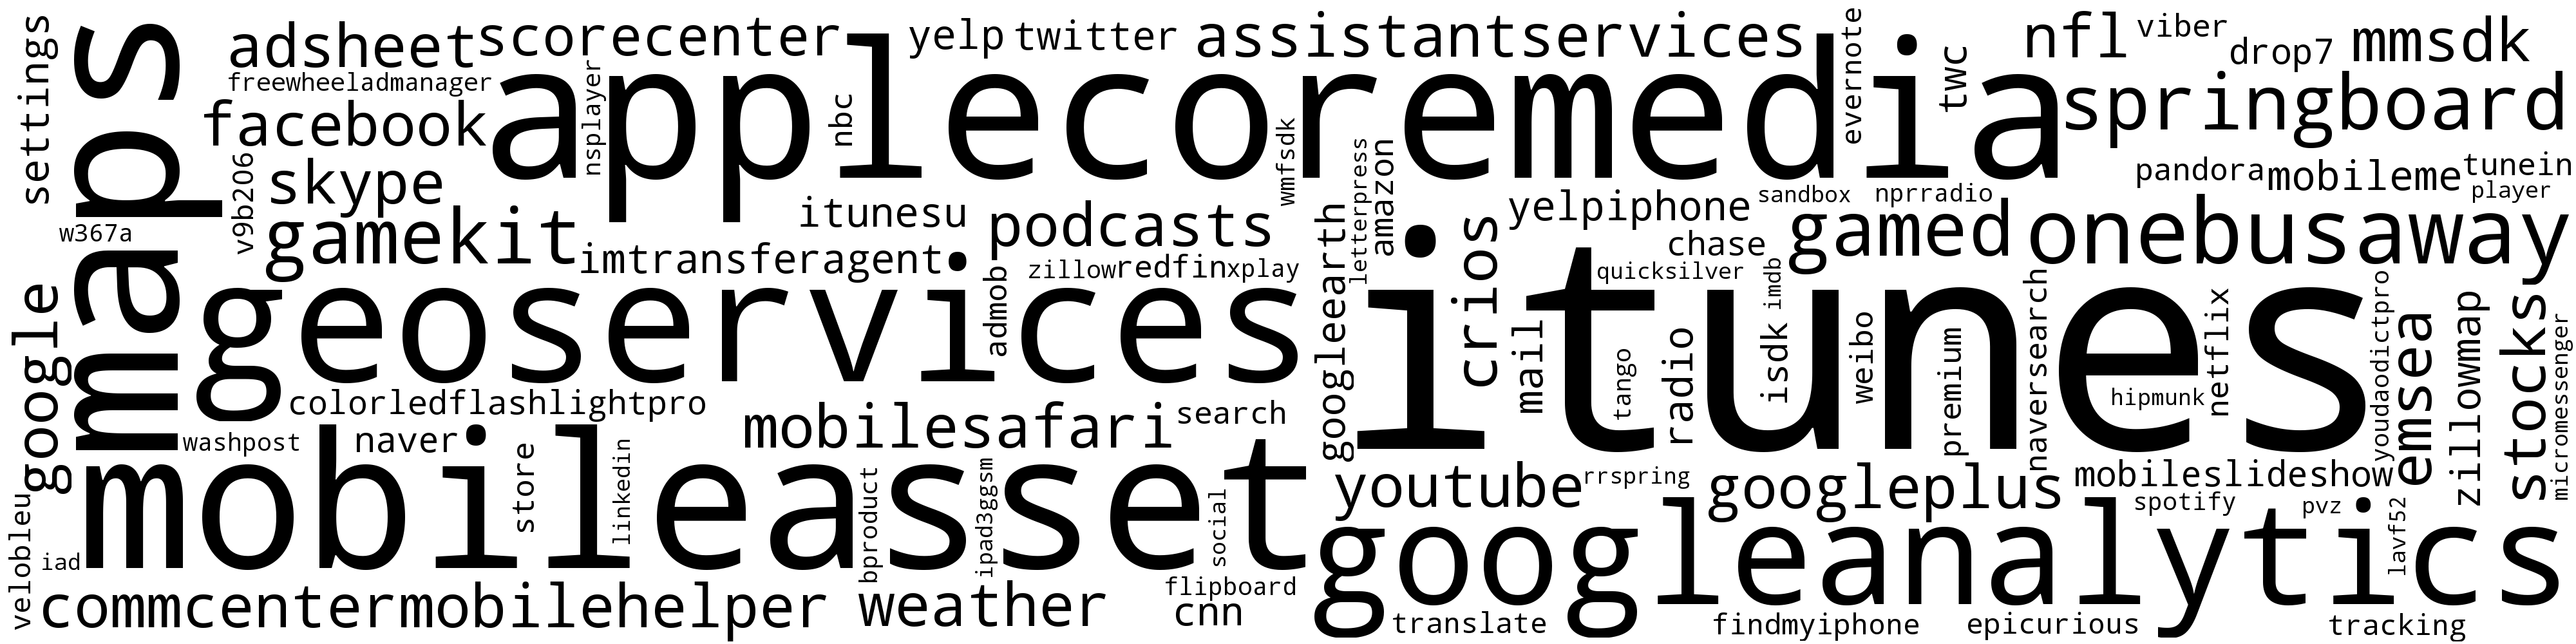
\includegraphics[width=\columnwidth]{figures/wordcloud_useragentsignature_ios_image.png}}\newline
\subfloat[Android]{\label{fig:http-wordcloud-android}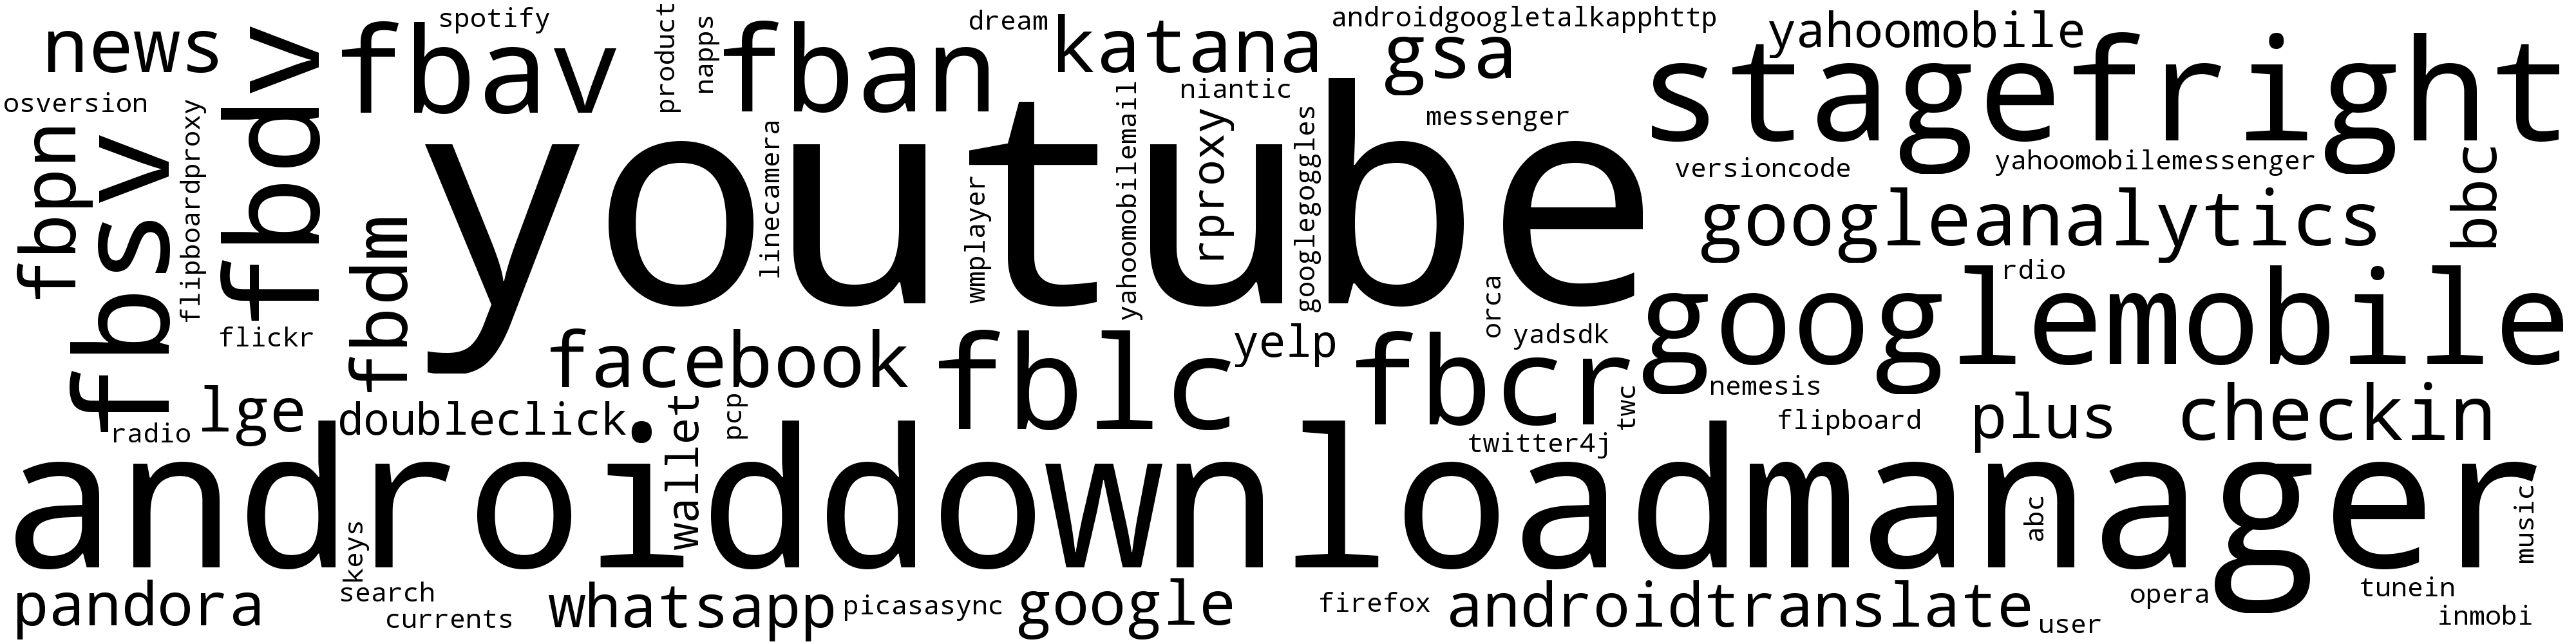
\includegraphics[width=\columnwidth]{figures/wordcloud_useragentsignature_android_image.png}}
\caption{\textbf{\useragent signatures in  iOS and Android HTTP flows.} \emph{The font weight represents the number of users for which a particular signature was observed.}}
%\vspace{\postfigspace}
\label{fig:http-wordcloud}
\end{figure}

%We now describe the results of classifying HTTP traffic in the \mobWild dataset. %mapping data gathered from our user study.
%Using only the \useragent on the \mobWild dataset, we were able to identify 256 iOS and 86 Android apps, OS libraries, and services. 
%The \emph{word cloud} in Fig.~\ref{fig:http-wordcloud} contains the summary of our results; the font size of an app/service name is proportional to the number of users for which it was observed.
%Note that \emph{Apple Core Media} and \emph{Stagefright} are services for downloading media content on iOS and Android devices, respectively.
%For the iOS devices in the \mobWild dataset, we observe a signature of \emph{Apple Core Media} in more than 98.45\% of the content downloaded from the YouTube servers (identified by their \httphost field).
%Similarly, we observe that YouTube flows contain ``Stagefright'' in HTTP headers. % to Android devices depending on the OS version. 
%We observe a similar signatures for other popular media services such as Netflix, YouTube, Vimeo, Pandora, etc, so we use the \httphost field to identify these Web services.
%\drc{AM: Suggests removing word cloud. PG doesn't like them either.}

\begin{table}
\centering
\begin{small}
\begin{tabular}{|p{0.15\columnwidth}|p{0.2\columnwidth}|c|c|c|c|}
\hline
\multirow{2}{*}{\bf Technique}&\multirow{2}{*}{\bf Category} & \multicolumn{2}{c|}{\bf iOS} &  \multicolumn{2}{c|}{\bf Android} \tabularnewline
\cline{3-6}
&   & {\bf Bytes}  & {\bf Flows} & {\bf Bytes} & {\bf Flows}   \tabularnewline
&   & {\bf (\%)}  & {\bf (\%)} & {\bf (\%)} & {\bf (\%)}   \tabularnewline

\hline
\multirow{2}{*}{\useragent} &Apps             & 43.21  & 85.73 & 15.01 & 75.17 \tabularnewline
\cline{2-6}
                            & OS Services$^{*}$            &  0.19  & 3.82 & 17.42 & 0.81 \tabularnewline
\hline
\useragent + &Media (Popular)         & 51.36  & 7.12  & 61.98 & 3.56 \tabularnewline
\cline{2-6}
\httphost  &Media (Other)           & 4.90  &  0.85 &  0.68 &  0.12 \tabularnewline
\hline
\httphost & Other Apps/Web-services  & $<$0.01 & 0.49 & 1.53  & 12.98 \tabularnewline
\hline
\multicolumn{2}{|c|}{Total Classified}  & {\bf 99.6} & {\bf 98.01} & {\bf 96.62} & {\bf 92.64} \tabularnewline
\hline
\end{tabular}
\end{small}
\caption{\textbf{Effectiveness of mapping HTTP traffic}. \emph{OS services$^{*}$ includes services other than those used to download media content.}}
\label{tab:classify-http}
\end{table}

\textbf{In situ data.}
Table~\ref{tab:classify-http} shows that a combination of \useragent and \httphost field in HTTP headers can map more than 92\% of the traffic (flows and bytes) from iOS and Android devices.

Using only the \useragent on the \mobWild dataset, we were able to identify 256 iOS and 86 Android apps, OS libraries, and services. 
We observe that the \useragent is more effective in identifying iOS apps compared to Android apps, which concurs with what we observed during our controlled experiments.

The \emph{word cloud} in Fig.~\ref{fig:http-wordcloud} contains the signatures we extracted from the \useragent; the font size of an app/service name is proportional to the number of users for which it was observed.
Signatures such as facebook and youtube are useful in identifying the apps, Facebook and YouTube respectively.
However, signatures such as applecoremedia and stagefright represent the OS services provided by iOS and Android to download media content which are internally used by media streaming apps such as Pandora and YouTube.
Audio and video streaming apps such as Pandora and YouTube use the \emph{Apple Core Media} and \emph{Stagefright} services on iOS and Android respectively to download media content, and for other auxiliary content such as list of related videos and recommendations these apps use the \useragent that contains their app signature.
We therefore use a combination of \useragent and \httphost field to identify such apps.

In Table~\ref{tab:classify-http}, we observe that media from popular streaming services---Netflix, YouTube, Pandora, Spotify, and Vimeo---contribute to more than 50\% of the traffic volume from iOS and Android devices in the \mobWild dataset.
We also observe that unmapped media served from CDNs and others hosts comprises less than 5\% of the traffic volume for the iOS and Android devices. 
We also observe that the \httphost field is more useful to classify Android traffic compared to iOS traffic, which concurs with what we observed during our controlled experiments. 

To summarize, by using a combination of \useragent and \httphost we were able to classify more than 92\% of the iOS and Android traffic by flows and bytes. 
%\drc{From PG: How is mapping to organization done?}

\subsubsection{SSL Traffic Mapping without Decryption}

SSL flows provide limited information in plaintext to identify apps. 
For the traces captured during our controlled experiments, we use SSL bumping to map HTTP flows using the techniques described in the previous section. 
However, we did not perform SSL bumping for the devices in the \mobWild dataset, so we now describe how to 
map SSL flows \emph{without decryption}. 

\noindent\textbf{Overview of mapping technique.}
Using port numbers, we observe in that more than 98\% of SSL flows observed in our controlled experiments were due to HTTPS, the rest of the flows were due to email, instant messaging, and OS notification services. 
We therefore focus our attention on identifying the apps responsible for the HTTPS flows.
We use DNS responses and subsequent SSL handshakes to determine the \emph{hostnames} of the remote hosts contacted by mobile devices.
After identifying the hostnames, we try to map these hostnames to apps using the technique described in the previous section.

%During manual examination of the results, we observe that Google and Apple to the be two main groups of organizations: Google and Apple.

% After identifying a hostname, we map the corresponding traffic in two phases.
% In the first phase we use the port number and hostname to identify the service 
% and group the traffic based on service. \drc{Why are you using the term ``service'' instead of app? 
% Why is this classification so different from the previous section? Need to make it more uniform.}
% The five most popular groups that we found in our dataset are social network, mail, media, instant messages, and notification.
% For example, flows to \url{facebook.com}, \url{twitter.com}, \url{plus.google.com} are grouped as social networks.
% Traffic to well known email ports such as TCP port 993, and traffic to hosts such as \url{mail.google.com} are classified as mail traffic.
% Similarly, we use documented ports to identify notification services (Android push) and instant messages (Facebook Messenger).

% In the second phase, we group hostnames that do not contain details of Web services.
% For example, the hostname \url{fbcdn-photos-a.akamaihd.net} indicates that the traffic is due to Facebook (due to \emph{fbcdn}), while \url{www.googleapis.com} hides the underlying app.
% We group hostnames that hide the app and Web service based on the parent organization.
% During manual examination of the traces, we observe two main groups: Google Services and Apple Services.
% Google Services includes flows whose remote hosts are served by Google, \eg \url{www.googleapis.com}, while Apple Services includes flows to servers managed by Apple, \eg \url{*.phobos.apple.com}
% This mapping, though crude, gives insights on the key sources of SSL traffic.

\noindent\textbf{Identifying hostname using the SSL Handshake.}
We first use the common name (CN) field of certificates to identify the servers that exchanged data using HTTPS.
We observe that less than 25\% of the HTTPS traffic from iOS and Android contains the fully qualified domain name (FQDN) in the subject of the certificate; the rest of the traffic either contains regular expressions such as *.google.com or is a continuation of a previous SSL session. 
To further resolve the hostnames, we rely on the \emph{Server Name Indication} (SNI) used by SSL flows~\cite{rfc:servernametls}.
Servers that host multiple services use the SNI to distinguish these services.   
For example, we observe an SNI of \url{plus.google.com} and \url{s.youtube.com} in two flows that used a certificate with a CN \url{*.google.com}.
Using either the certificate or the SNI we were able to identify the hostname for less than 40\% of HTTPS traffic.

\noindent\textbf{Identifying hostname using the DNS messages.} 
For the remaining flows we use DNS messages exchanged by the mobile device with its DNS server before starting the HTTPS flows, a technique similar to DN-Hunter~\cite{bermudez:dnhunter}.
DN-Hunter relies on the most recent FQDN that corresponds to the IP address, however in our controlled experiments we observe Android and iOS devices use the first entry in DNS response while resolving hostnames.
We therefore use the latest DNS response that contains the IP address of the Web service in the first position.
In spite of the potential usefulness of DNS responses, we give a high priority to the SNI and the certificates because the DNS response differs from these in 9.2\% of the iOS traffic and 5.6\% of Android traffic.
This difference is due to caching of DNS responses by the apps.

% \begin{table}
% \centering
% \begin{small}
% \begin{tabular}{|p{0.1\columnwidth}|p{0.2\columnwidth}|c|c|c|c|}
% \hline
% \multirow{2}{*}{\bf Phase} & \multirow{2}{*}{\bf Category} & \multicolumn{2}{c|}{\bf iOS Traffic} &  \multicolumn{2}{c|}{\bf Android Traffic} \tabularnewline
% \cline{3-6}
%  &         & {\bf Bytes}  & {\bf Flows} & {\bf Bytes} & {\bf Flows}   \tabularnewline
%  &         & {\bf (\%)}  & {\bf (\%)} & {\bf (\%)} & {\bf (\%)}   \tabularnewline
% \hline
% \multirow{5}{*}{Apps (A)}
% & Social Ntwks    & 12.81 &  7.74 & 35.39 & 19.28 \tabularnewline
% \cline{2-6}
% & Mail               &  6.11 &  9.26 &  6.46 & 11.02 \tabularnewline
% \cline{2-6}
% & Media              &  0.94 &  0.25 &  3.66 &  3.62 \tabularnewline
% \cline{2-6}
% & Instant Msg   &  3.70 & 14.09 &  0.21 &  0.48 \tabularnewline
% \cline{2-6}
% & Notifications     &  4.69 & 17.45 &  2.02 &  6.57 \tabularnewline
% \cline{2-6}
% %\hline
% & \emph{Total (A) }       & {\em 28.25} & {\em 48.79} & {\em 47.74} & {\em 40.97} \tabularnewline
% \hline
% \multirow{2}{*}{Organization (B)}
%  & Google Svcs   & 36.32 & 17.56 & 47.31 & 48.27 \tabularnewline
% \cline{2-6}
%  & Apple Svcs    & 25.26 & 28.26 & $<$0.01 & $<$0.01 \tabularnewline
% \cline{2-6}
% \cline{2-6}
% & \emph{Total (B) }       & {\em 61.58} & {\em 45.82} & {\em 47.31} & {\em 48.27} \tabularnewline
% \hline
% \multicolumn{2}{|c|}{\emph{Total (A + B)}}       & {\em \bf 89.83} & {\em\bf 94.61} & {\em\bf  96.10}  &  {\em\bf  89.24} \tabularnewline
% \hline
% \end{tabular}
% \end{small}
% \caption{\textbf{Mapping SSL traffic in the \mobWild dataset.} \emph{The iOS and Android SSL traffic in the \mobWild dataset is dominated by Google and Apple Services. The share of Social Network traffic is higher for Android devices because the default photo backup services on Android devices uses the Google Plus (and Picasa) Social Network.}}
% \label{tab:classify-ssl-traffic}
% \end{table}



\begin{table}
\centering
\begin{small}
\begin{tabular}{|p{0.3\columnwidth}|c|c|c|c|}
\hline
\multirow{2}{*}{\bf App/Org} & \multicolumn{2}{c|}{\bf iOS Traffic} &  \multicolumn{2}{c|}{\bf Android Traffic} \tabularnewline
\cline{2-5}
                              & {\bf Bytes}  & {\bf Flows} & {\bf Bytes} & {\bf Flows}   \tabularnewline
                              & {\bf (\%)}  & {\bf (\%)} & {\bf (\%)} & {\bf (\%)}   \tabularnewline
\hline

Apps            & 28.25 & 48.79 & 47.74 & 40.97 \tabularnewline
\hline
Google Services & 36.32 & 17.56 & 47.31 & 48.27 \tabularnewline
\hline
Apple Services  & 25.26 & 28.26 & $<$0.01 & $<$0.01 \tabularnewline
\hline
{\emph{Total}}  & {\em \bf 89.83} & {\em\bf 94.61} & {\em\bf  96.10}  &  {\em\bf  89.24} \tabularnewline
\hline
\end{tabular}
\end{small}
\caption{\textbf{Mapping SSL traffic in the \mobWild dataset.} \emph{The SSL traffic from the iOS and Android devices in the \mobWild dataset is dominated by Google and Apple services.}}
\label{tab:classify-ssl-traffic}
\end{table}

\noindent\textbf{Mapping results.} 
Table~\ref{tab:classify-ssl-traffic} shows our SSL mapping results on the SSL traffic in the \mobWild dataset. 
We first group hostnames to the apps and we were able to identify the apps for more than 40\% of the iOS and Android SSL flows.
For flows whose hostnames are ambiguous, we group them according to organizations.
During manual examination of the results, we observe that Google and Apple to be the two main organizations that contributed to the majority of the flows; we label these flows as Google Services and Apple services respectively. 

In Table~\ref{tab:classify-ssl-traffic}, we observe that 61.5\% of iOS and 47.3\% of Android traffic (by bytes) is respectively 
to Google and Apple servers where the hostname does not contain signatures of the app.
This share does not include the traffic to Google and Apple servers that we classified as apps.
For example, flows to \url{mail.google.com} were classified as GMail and are placed in the category apps, while flows to \url{www.googleapis.com} is categorized as Google Services. 
Google services and Apple services are therefore the largest sources of SSL traffic in our \mobWild dataset.

In summary, using the certificates, SNI, and DNS messages, we were able to identify the hostname of the remote hosts for more than 89\% of the SSL flows.
We observe that Google and Apple are the dominant sources of SSL traffic for the Android and iOS devices in the \mobWild dataset.

\subsubsection{Summary}

We use the a combination of \useragent and \httphost field to identify apps responsible for HTTP flows.
On applying our technique to the \mobWild dataset, we were able to classify more than 92\% of the iOS and Android traffic by flows and bytes. 
We observe that the \useragent field is more effective to identify HTTP flows from iOS devices compared to Android devices.
We speculate that this behavior is because of the strict coding practices mandated by Apple while packaging iOS apps~\cite{xcode:distrib}.

We use certificates, SNI, and DNS messages to map SSL flows, and we were able to classify more than 90\% of SSL traffic in the \mobWild dataset using our classification technique. 
To the best of our knowledge, we are the first to study the effectiveness of these fields in classifying SSL flows from mobile devices.

%%% Local Variables: 
%%% mode: latex
%%% TeX-master: "main"
%%% End: 




%\section{Measurements}
%\label{sec:measurements}

\eat{All the subsections are now sections. We can merge them later}

\section{Network Characteristics of Notification Services}
\label{sec:characterize-os}

Mobile operating systems provide OS level notification services to optimize network usage.
The Apple Push Notification service (APNs) and Google Cloud Messaging (GCM)~\cite{gcm} are used by iOS and Android applications respectively to receive notifications from the Internet.
In this section we show how \platname was used to compare the notification services of iOS and Android, and detailing it behavior in the wild. 

\begin{figure}
\centering
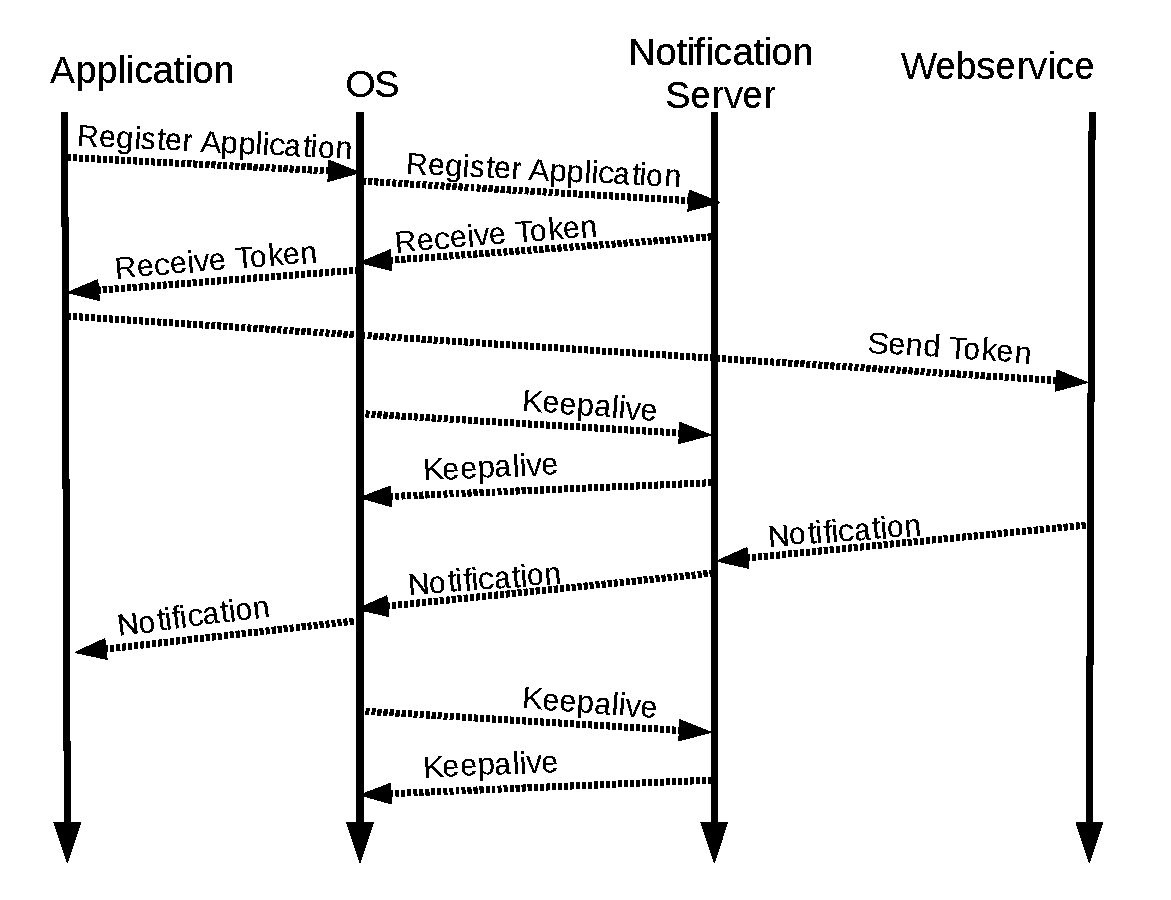
\includegraphics[width=\columnwidth]{figures/Notification.pdf}
\caption{Notifications on mobile OSes. \emph{Because notification messages are sent over TCP, keepalive messages are periodically exchanged to ensure TCP connections do not timeout.}}
\label{fig:push-expt-interarrival}
\end{figure}



\subsection{Controlled Experiment on Factory Reset Devices}

We first detail the detail the behavior of notification services by performing a controlled experiment on \emph{factory-reset} devices. 
The objective of this experiment was to analyze notification services for devices that are used \emph{out of the box}, and detail the impact of device manufacturer, and pre-installed applications. 

For our experiment, we performed a \emph{factory reset} on an iPod Touch, an iPad, an iPhone, a Samsung Galaxy SIII, and a Google Nexus S Phone; the reset was performed after their batteries were fully charged. 
We then perform the initialization step and assigned a dummy email account as the primary account to each of these devices.
We then allowed these devices to connect to the Internet over \wifi through \platname and monitored the Internet traffic from these devices.
We then studied the impact of access technology by letting the iPhone and Samsung Galaxy SIII tunnel traffic through \platname using cellular networks. 

We observed that the traffic volume during the 24 hour periods varied from 19~KB to 97~KB depending on the devices. 
We classify APNS and GCM messages using the TCP port numbers mentioned in their specifications~\cite{gcm, apns}.
Because we did not run any applications in the foreground, notification messages were responsible for largest fraction of the traffic volume; the share was 35\% for Nexus S, 88\% for the Samsung SIII and around 50\% for each of the iOS devices. 
The share of DNS traffic varied from 10\% to 40\% for each of the devices while the other services contributed to less than 10\% of the traffic volume.
The only exception was the Samsumg Galaxy SIII which used location services that contributed to 26\% of 47~KB traffic volume generated by the device.

\begin{figure}
\centering
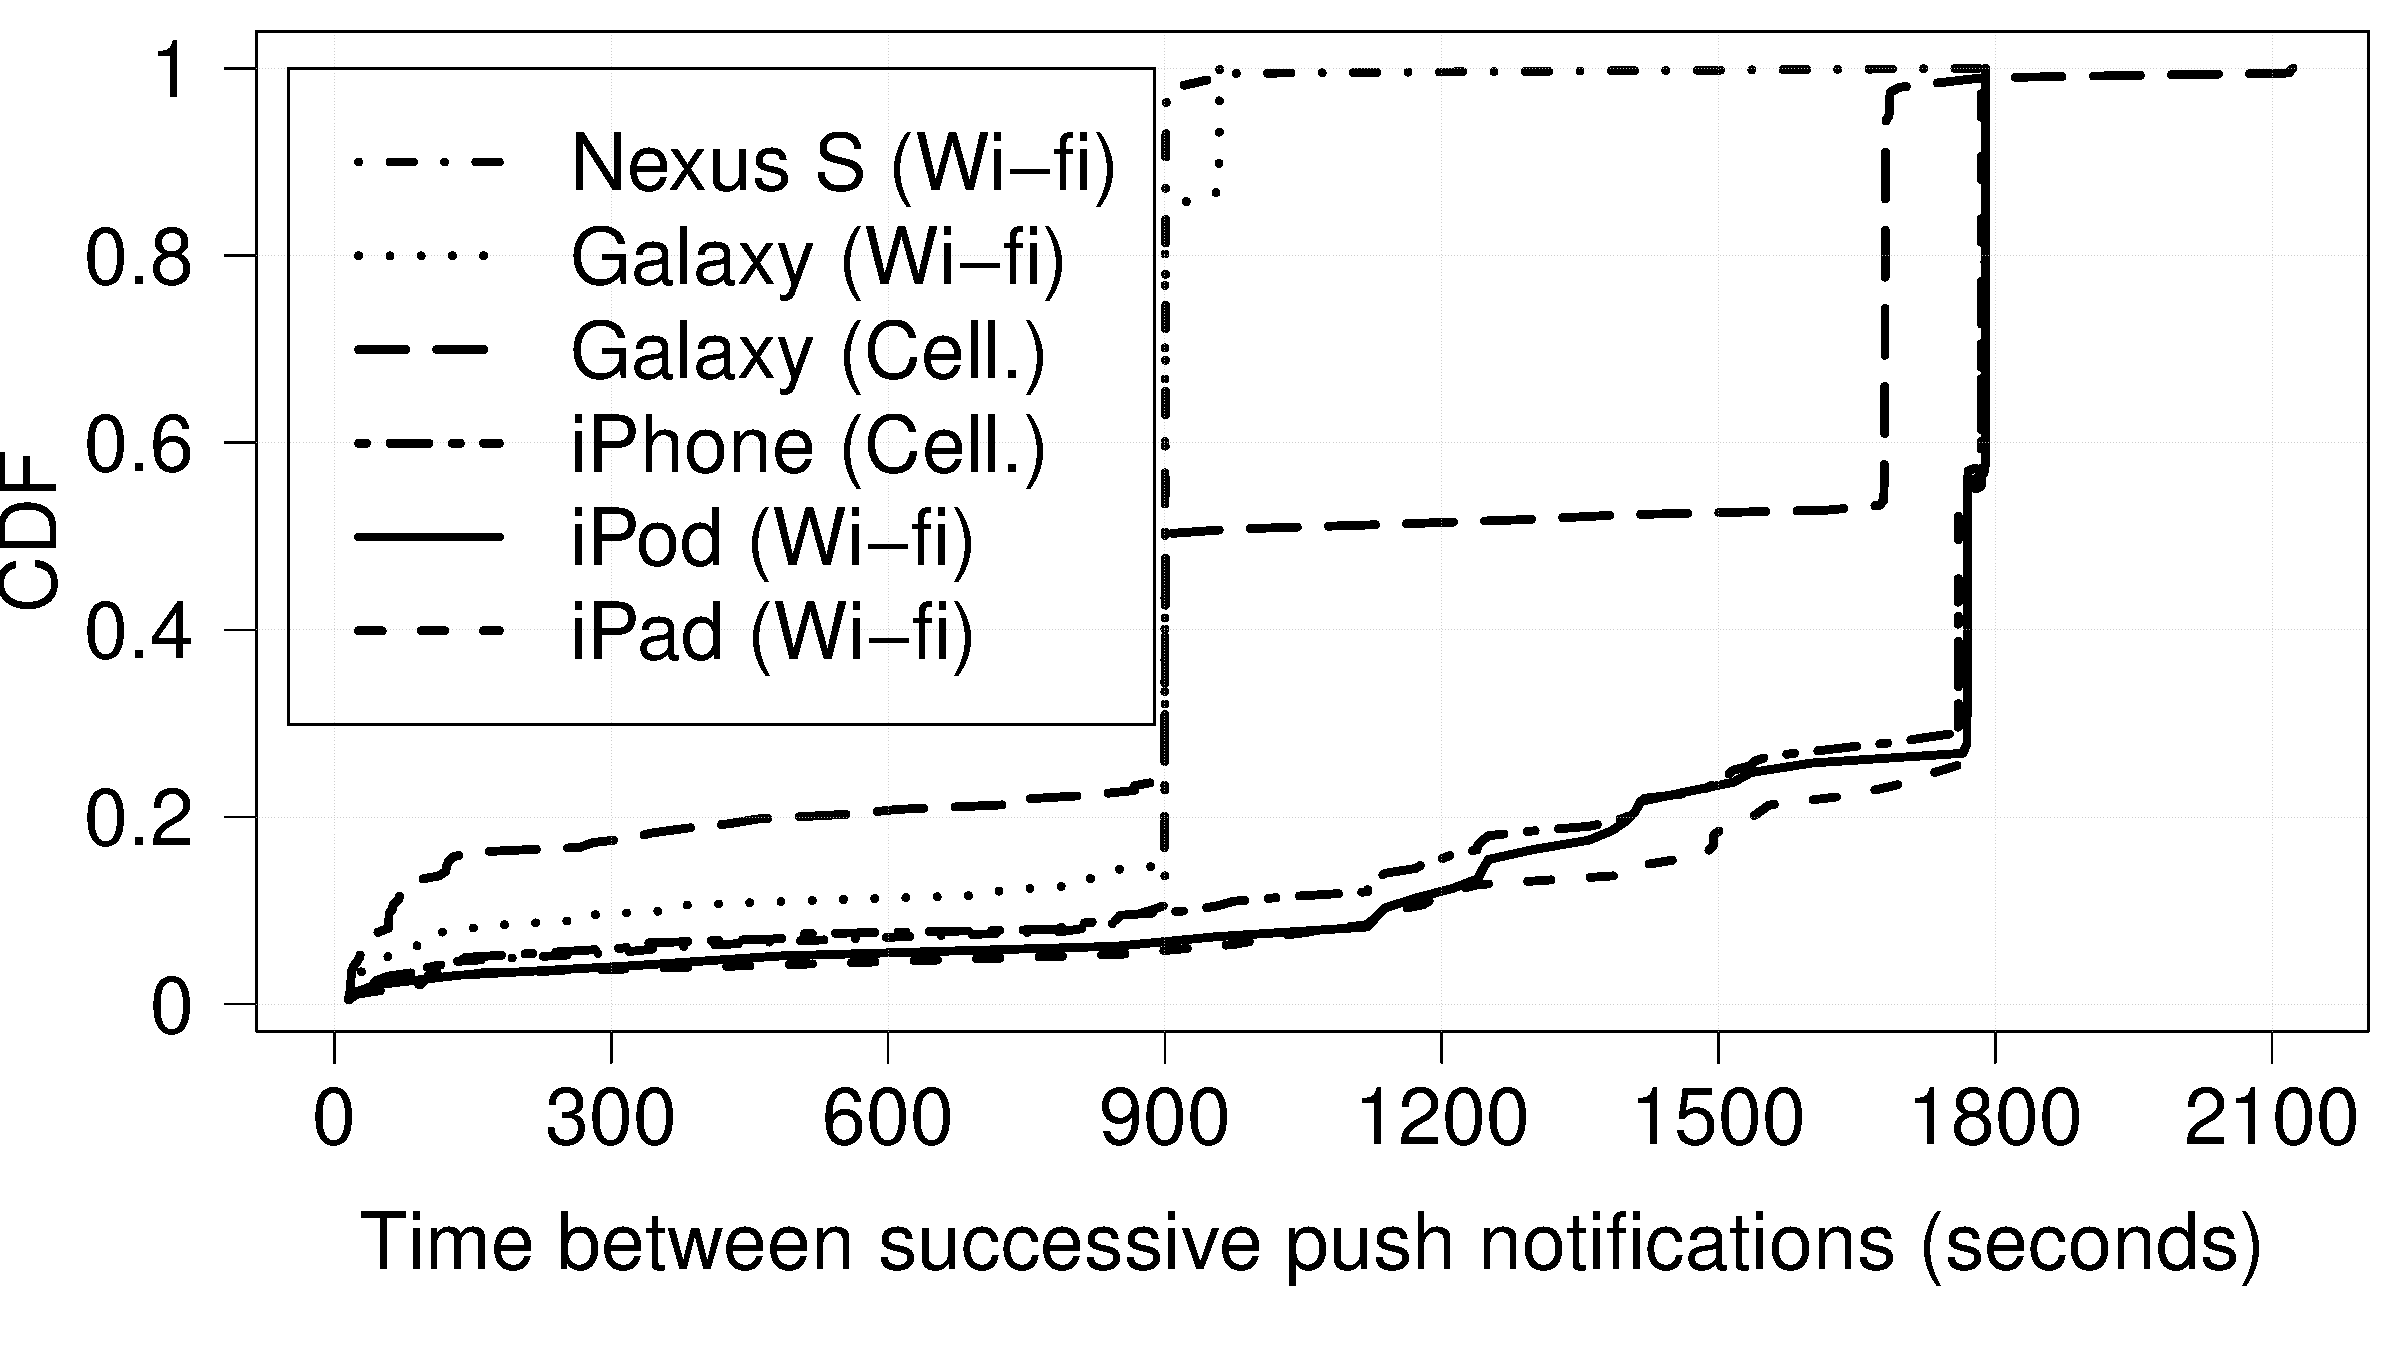
\includegraphics[width=\columnwidth]{plots/push_factoryreset_interarrival_distrib.pdf}
\caption{Inter-arrival time between notification messages after factory reset. \emph{The Android and iOS devices communicate with the notification server approximately once every 900~seconds and 1800 seconds respectively. The behavior of Android devices depends on the device, the pre-installed applications, and the access technology.}}
\label{fig:push-expt-interarrival}
\end{figure}

In \fref{fig:push-expt-interarrival} plot the time between successive messages sent by the notification servers on the ports assigned for notifications. 
We observe that the inter-arrival time between notifications for the Android devices is at least 900 seconds for more than 80\% of the notifications observed. 
The distribution of the inter-arrival time also depends on the access technology for the Samsung Galaxy SIII phone; we observe steps in the distribution for the SIII phone while we do not observe these steps when the same phone uses \wifi. 
We do not observe this difference when the Nexus S phone used the cellular data connection; we do not present the figure due to lack of space. 
\tbd{AR: Why these difference -- which applications stop coming up and so on}.
For the iOS devices, we observe an inter-arrival time at least 1700~seconds for that more than 75\% of the notifications in \fref{fig:push-expt-interarrival}. 
We do not observe a significant difference between the inter-arrival times for the iPhone over cell and \wifi and we do not present these results due to lack of space. 

On analyzing the packets exchanged, we observe that  all Android flows with an inter-arrival time larger than 800 seconds consisted of an empty TCP packet sent by the device followed by a 25 byte payload sent by the server.
Similarly, all iOS flows with an inter-arrival time larger than 1500 seconds began with an TCP packet with a payload of 85 bytes sent by the device followed by the server responding with of a TCP packet of 37 byte payload.

In summary, we observe notifications consume very little data, less than 50~KB in 24 hours, on Android and iOS devices in their default state.
The large time between successive notifications and the small amount of data exchanged implies they consume very little power.
We also observe that iOS devices have a larger time between successive notifications compared to Android devices in the default state. 
Furthermore, the inter-arrival time between notifications for Android devices differs based on the device manufacturer and the access technology. 

\subsection{Notifications In The Wild} 

We now characterize our observations on the notifications we observed in the \mobWild dataset. 
The objective of this analysis was to detail the frequency, traffic volume, and source of the notification services. 

\begin{figure}
\centering
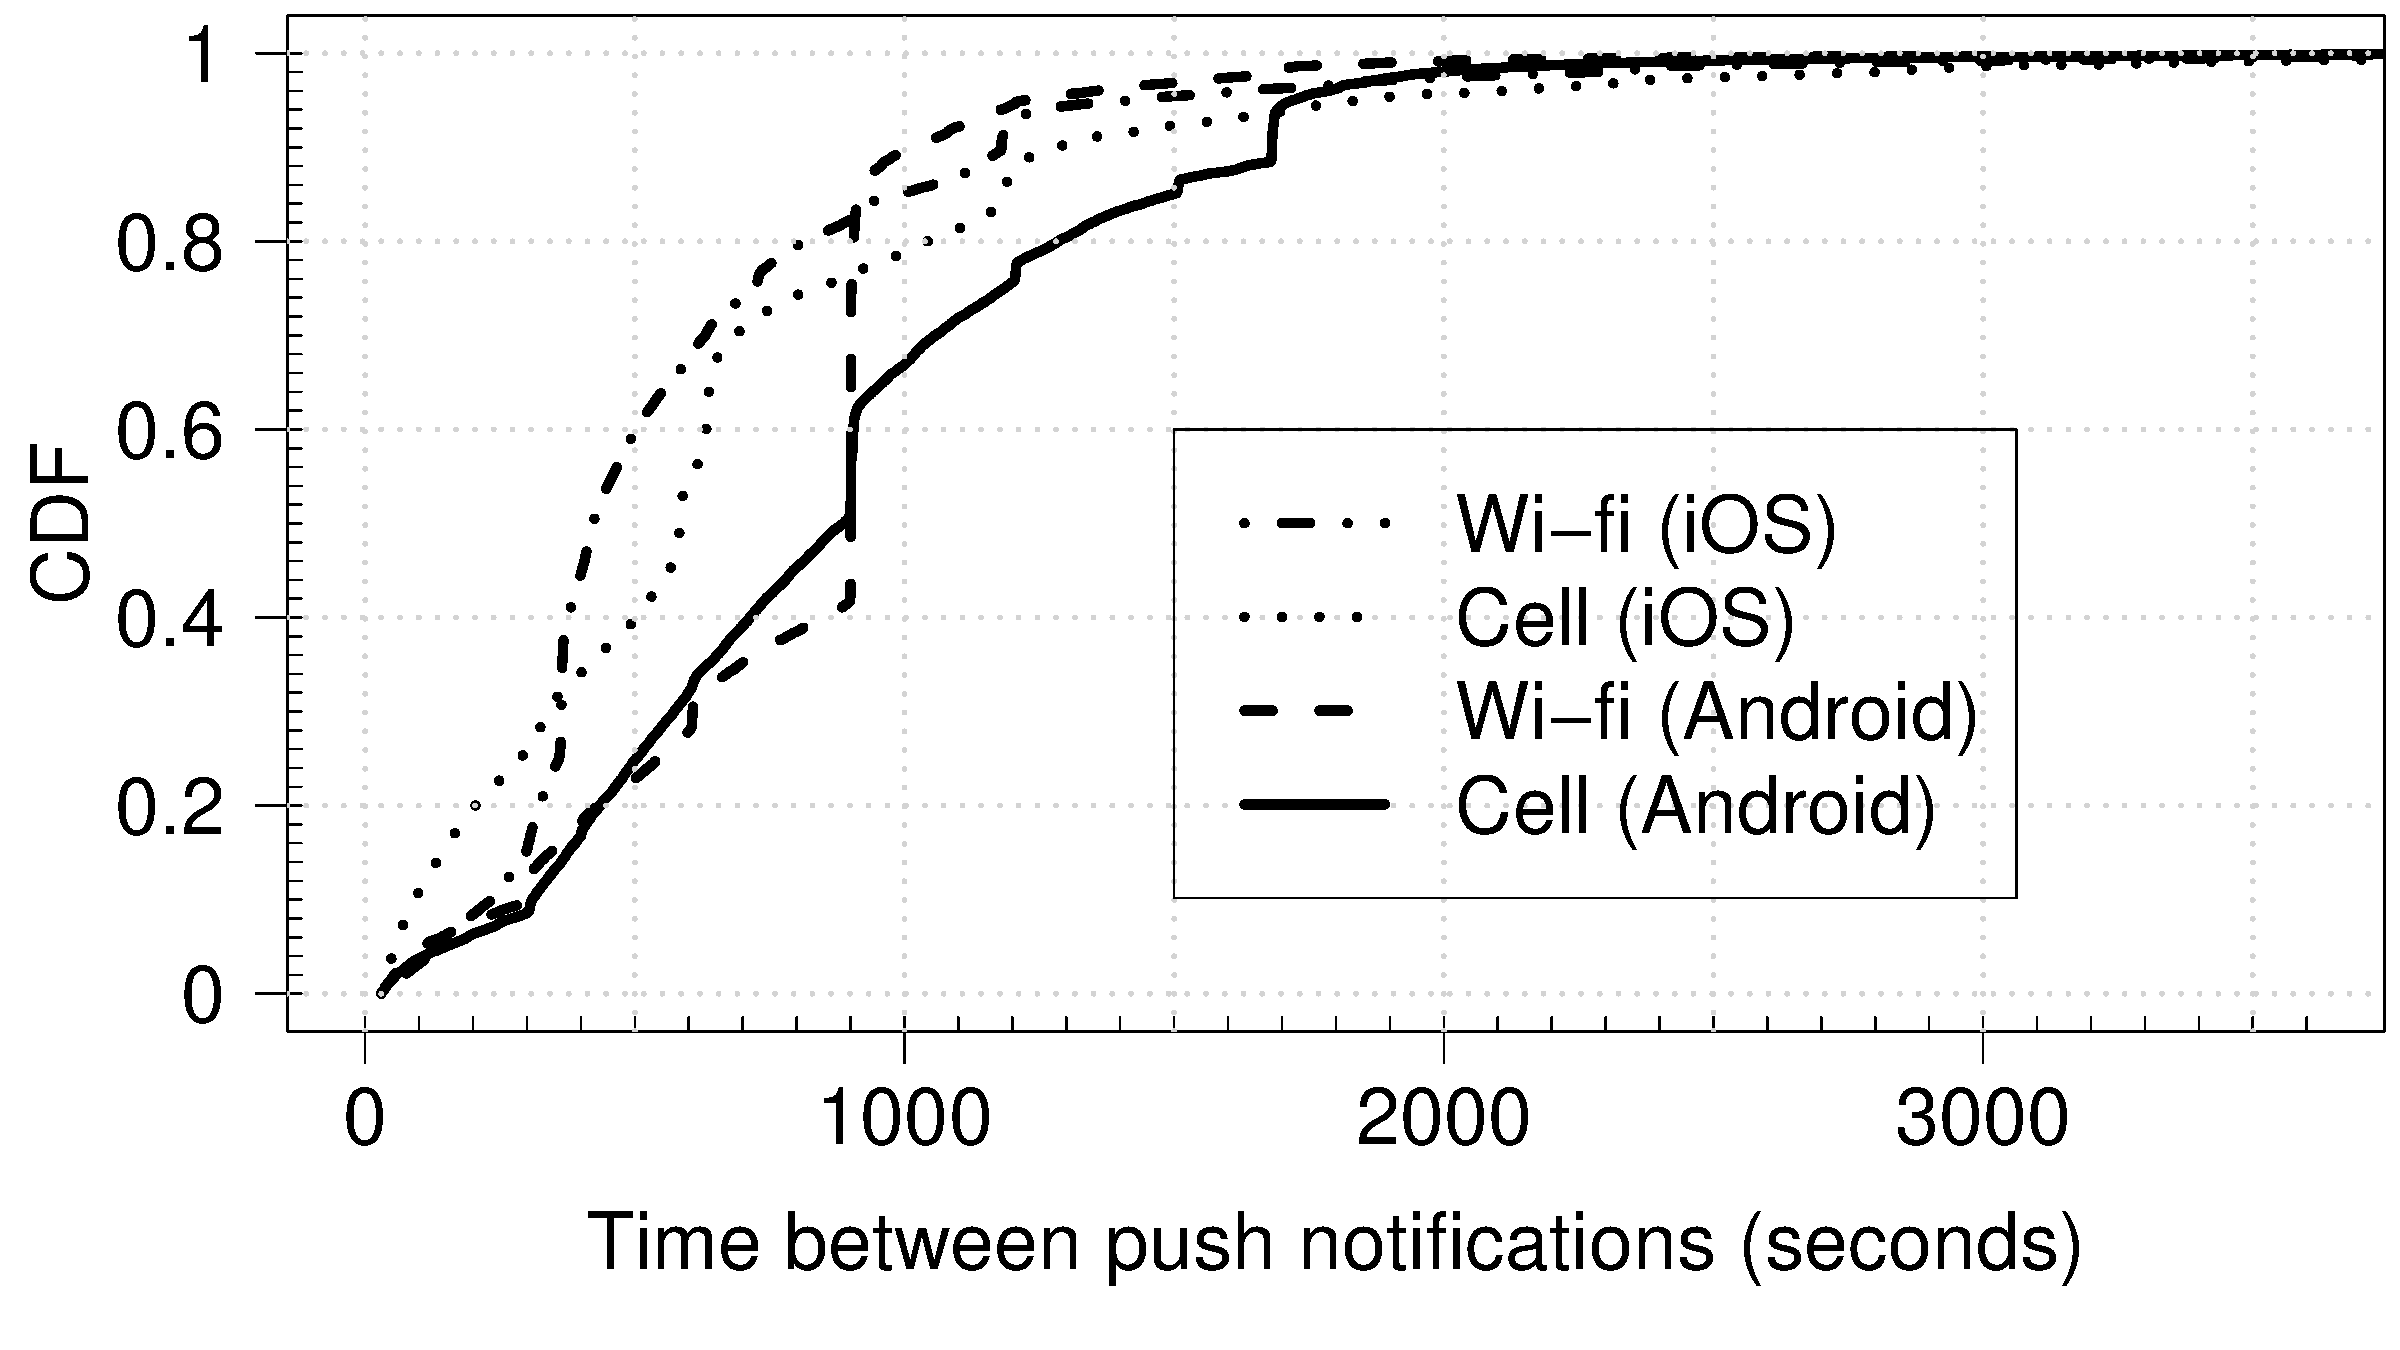
\includegraphics[width=\columnwidth]{plots/push_compare_os_tech_wild_distrib.pdf}
\caption{Distribution of the time between push notification messages in the wild. \emph{The frequency of push notification messages is higher for the iOS devices in our dataset compared to the Android devices. Notification messages are less frequent over cellular networks compared to Wi-Fi networks.}}
\label{fig:push-wild-compare-ostech}
\end{figure}

%The advantage of \platname is that it allows for direct comparison between devices across and their behavior across access technologies. 
To analyze the frequency of notification messages, we plot the distribution of the time between successive push notification messages for Android and iOS devices over cellular and \wifi networks in \fref{fig:push-wild-compare-ostech}.
In \fref{fig:push-wild-compare-ostech} we observe that a higher time between push notifications over cellular networks in comparison to \wifi networks for iOS and Android devices.  
We also observe the Android devices in our dataset receive notifications less frequently compared to the iOS devices in our dataset. 
We also observe a heavy tail for the time between notification messages which implies potentially long idle intervals.
\tbd{Correlation between time between notification messages and size of the next idle time observed?}


\begin{figure}
\centering
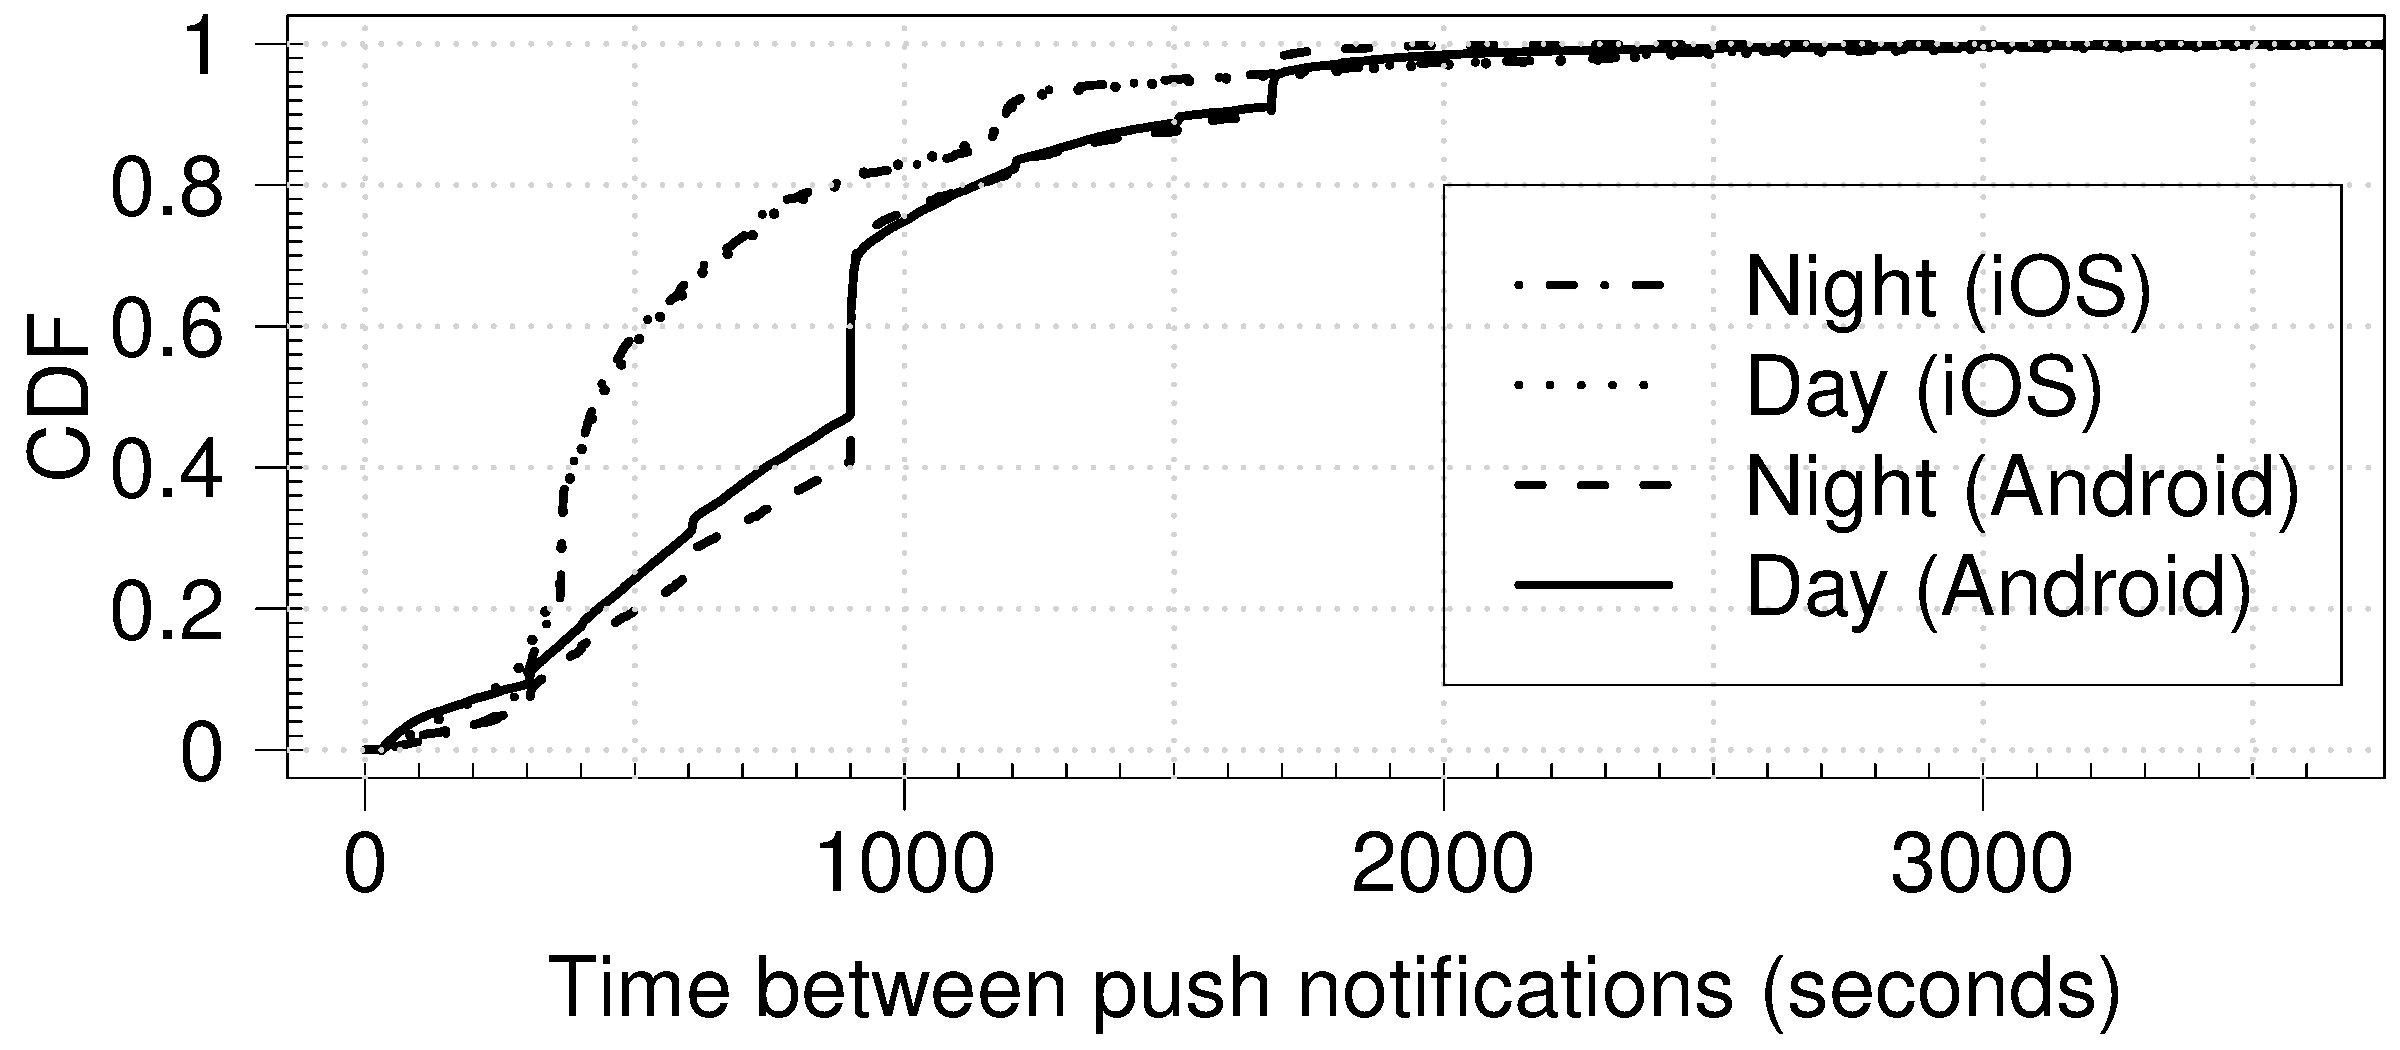
\includegraphics[width=\columnwidth]{plots/push_compare_diurnal_wild_distrib.pdf}
\caption{Impact of time-of-day on the push notifications. \emph{The rate of notifications is agnostic of the time of the day for iOS and Android devices.}}
\label{fig:push-wild-diurnal}
\end{figure}

The notification messages could be in response to user actions, for example, a mail server might receive a notification of a new message.
To analyze this impact, we notification messages received during two time intervals: from midnight to 6 am (night), and from 6 am to midnight (day). 
In \fref{fig:push-wild-diurnal}, we plot the distribution between successive notification messages for these two intervals. 
We observe that the Android and iOS devices appear to be agnostic of the time of the day. 
The iOS devices (from verion 6.0) come with a feature called \emph{Do Not Disturb (DND)} that does raise notification alarms on receiving notifications during specific time periods. 
We observe notification messages were received by the device that had enabled this feature during the intervals their users had configured as \emph{Do Not Disturb}.

\begin{figure}
\centering
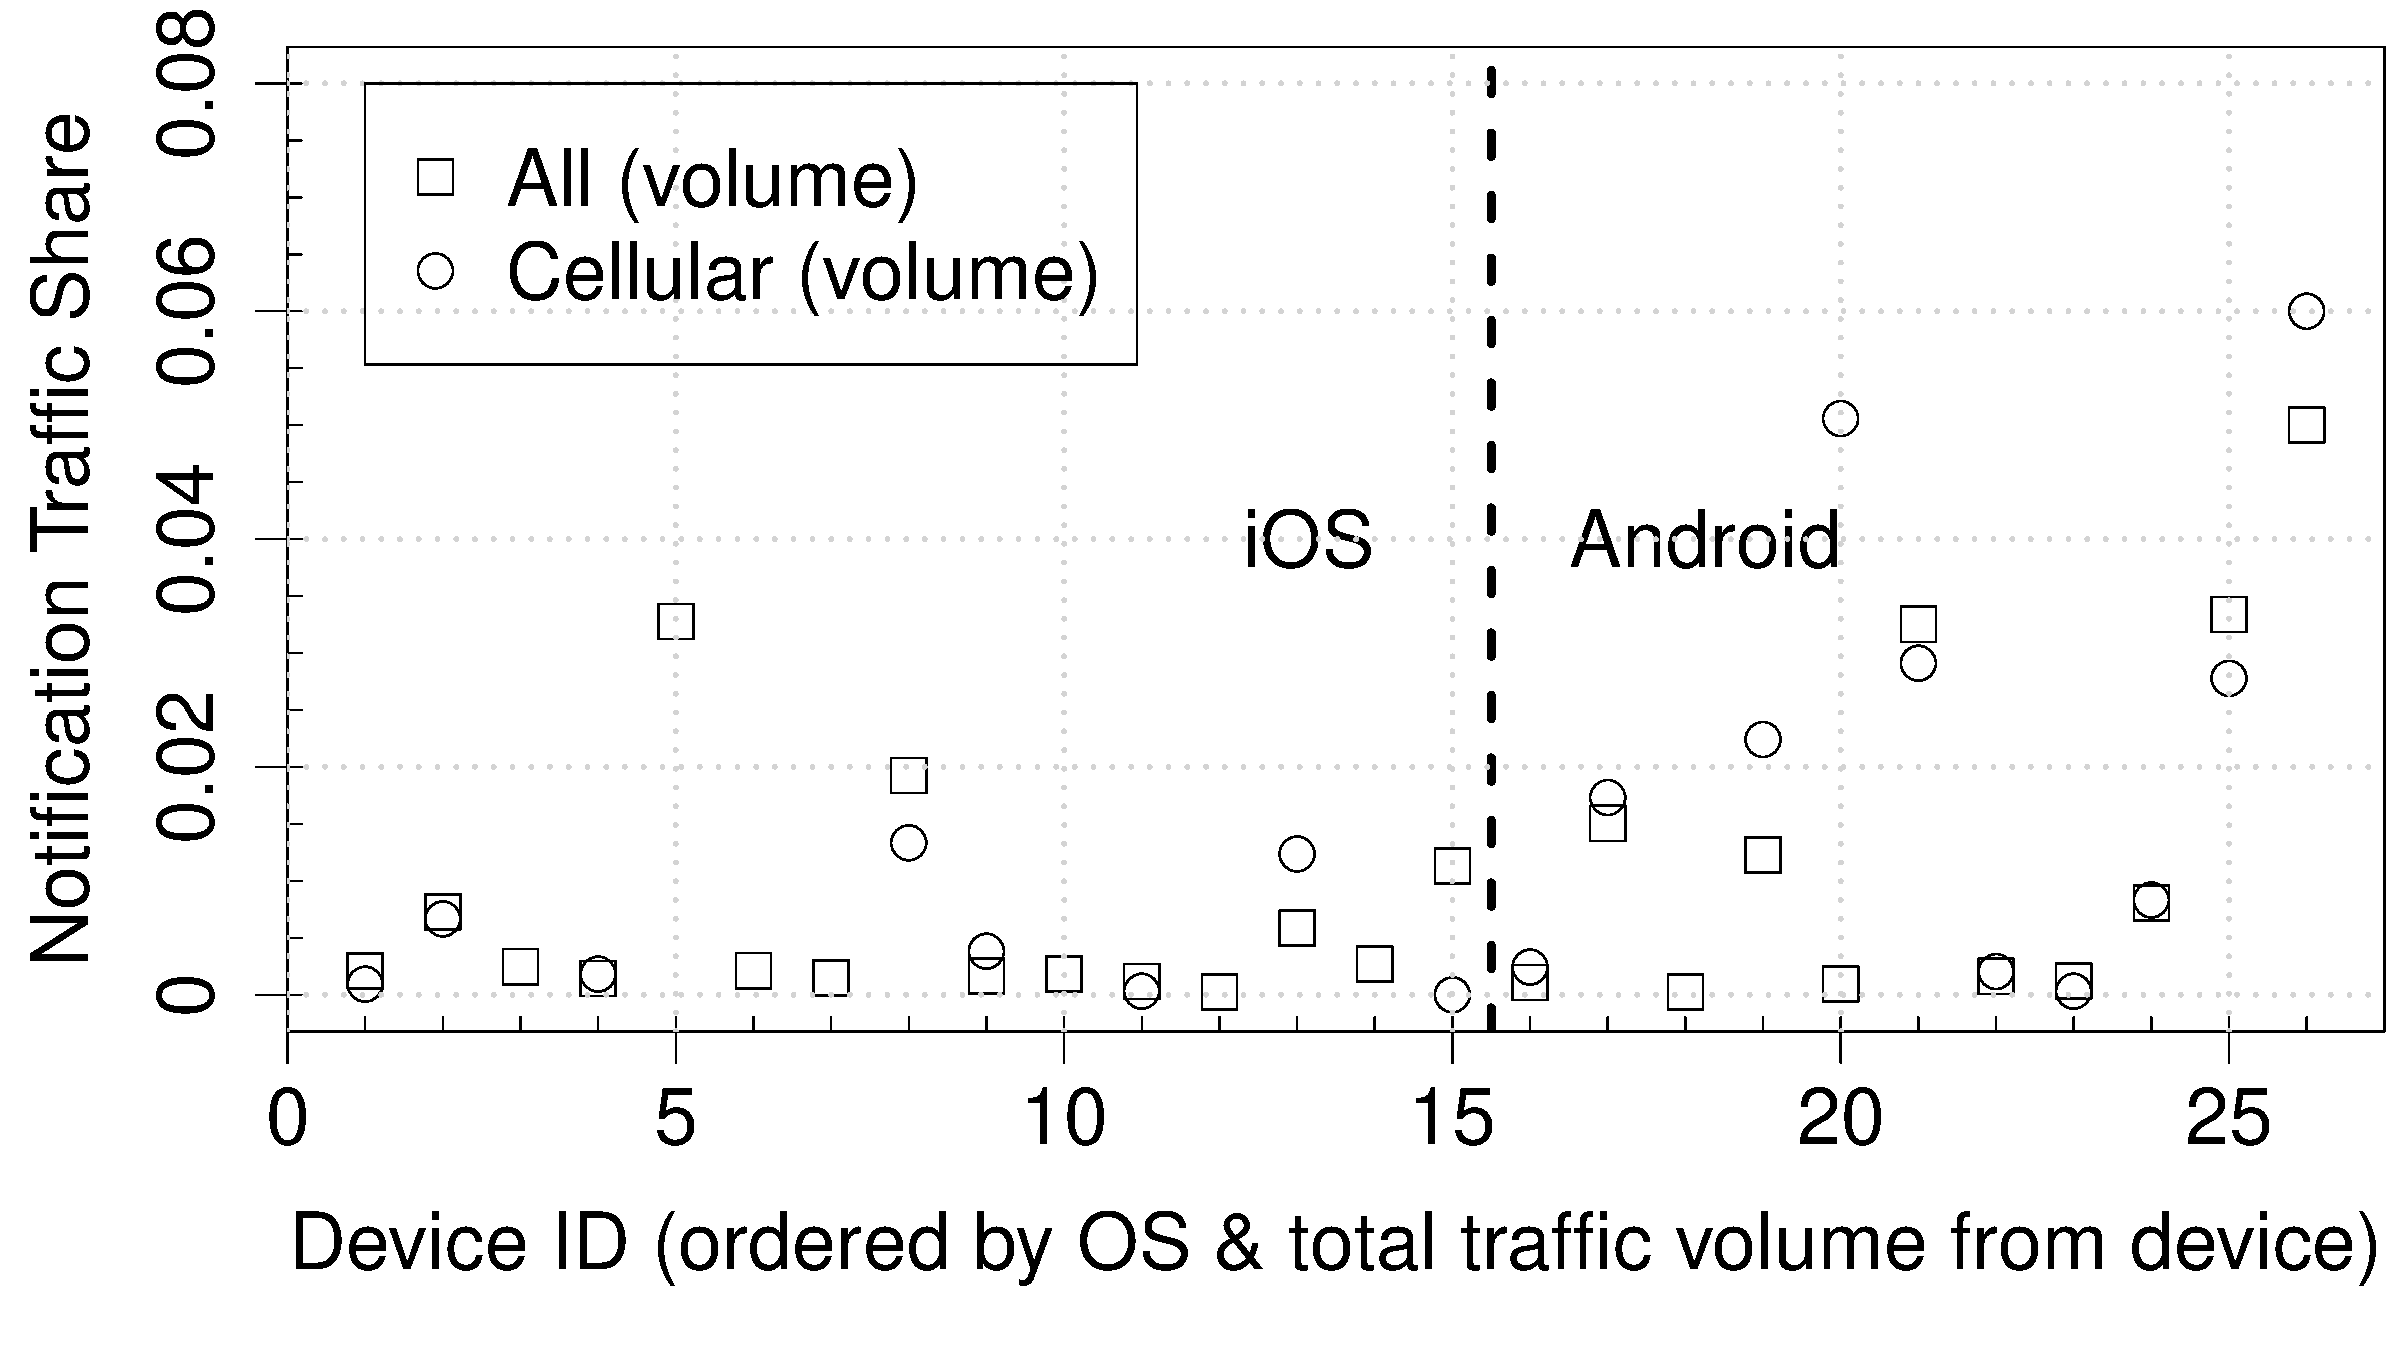
\includegraphics[width=\columnwidth]{plots/push_compare_trafficshare.pdf}
\caption{Traffic share of push notifications. \emph{Push notifications are responsible for less than 5\% of the traffic volume on most devices.}}
\label{fig:push-traffic-share}
\end{figure}

To analyze the volume of notification messages, we plot the share of notification messages as a fraction of total traffic from the device in \fref{fig:push-traffic-share}.
We observe that the notification messages are responsible for less than 4\% of the traffic volume on most Android and iOS devices. 
In \fref{fig:push-traffic-share}, we also plot the share of notification messages when the device exchanged data over cellular networks. 
We observe that there is no significant difference in the traffic share of notification messages when the device used cellular traffic. 
\tbd{Why do we care?}

To further analyze the source of the notification messages we analyzed the DNS lookups that were performed before the connections for receiving notification messages was established. 
We observed that the servers that pushed content to iOS devices correspond to the DNS requests that match the pattern \emph{*courier.push.apple.com} and \\ \emph{*courier-push-apple.com.akadns.net}.
For the android devices we observe that the DNS requests match the pattern\\ \emph{*talk.google.com}. 

In summary, we detail the behavior of the notification services using controlled experiments and the \mobWild dataset.  
We observe that push notifications consume a small fraction of the data and exhibit a heavy tail for the time between successive messages. 
We also observe that the frequency of notification messages was agnostic of the time of the day. 
Furthermore, notification messages were received by iOS devices even during the time interval the users had configured \emph{Do Not Disturb.}


% \begin{packedenumerate}
% \item How frequently do Push notifications take place in the wild?
% \item What is the impact of access technology on push notifications?
% \item What is the impact of the time of the day?
% \item What is the volume of push notification traffic?
% \item From which hosts are these notifications received?
% \end{packedenumerate}

%\subsection{Discussion}




% OLD TABLE WITHOUT IPHONE
% \begin{table}
% \begin{small}
% \begin{tabular}{|c|c|c|c|c|}
% \hline
% \multirow{2}{*}{\bf Application} & \multicolumn{4}{c|}{\bf Traffic Share in the first 24 hours}\tabularnewline
% \cline{2-5}
%      & iPad & iPod & Galaxy SIII & Nexus \tabularnewline
%      & (19 KB) & (21 KB) & (47 KB)& (97 KB)  \tabularnewline
% \hline
% Notifications & 0.54 & 0.53 & 0.35 & 0.88 \tabularnewline
% \hline
% Location & 0 & 0 & 0.26 & 0 \tabularnewline
% \hline
% SSL & 0 & 0 & 0.30 & 0.11 \tabularnewline
% \hline
% Mail & 0.05 & 0.07 & 0 & 0 \tabularnewline
% \hline
% HTTP & 0.13 & 0 & 0.09  & 0 \tabularnewline
% \hline
% UDP & 0.28 & 0.40 & 0.01 & 0.01 \tabularnewline
% \hline
% {\em total}& {\em 1.0} & {\em 1.0} & {\em 1.0} & {\em 1.0}\tabularnewline
% \hline
% \end{tabular}
% \end{small}
% \caption{Network usage in the first 24 hours after factory reset. \emph{Notifications contribute to the largest fraction of traffic volume across all devices.}}
% \label{tab:traffic-share-factory-reset}
% \end{table}

%While computing this distribution, we account the diversity in device usage in the following manner.
%For each device and each access technology we compute the 100 quantiles from 0.01 to 1.0 in steps of 0.01 of the time between successive push notifications. 
%We then use the median value of each quantile (from 0.01 to 1.0 in steps of 0.01) for a given access technology and operating system of the device.

% In \fref{fig:wild-inter-arrival-push} we present the time between successive push notifications for the 25 devices in our dataset. 
% As observed in \fref{fig:wild-cdf-push} we observe that the iOS devices receive push messages more frequently that the Android devices. 
% We also observe that the time between push notifications is higher for Android devices.
% The iOS devices prefer a cellular data connection for Push notification over \wifi \tbd{http://support.apple.com/kb/TS4264}. 
% However, in \fref{fig:wild-cdf-push} and \fref{fig:wild-cdf-push} despite this preference, we observe that the time between successive push notifications for iOS devices is higher over cellular networks in comparison to \wifi networks.  
% We observe that \tbd{SSL traffic} to mail servers was followed \tbd{x\%} after push notifications.
% This implies that higher usage of the device over \wifi may result in a higher number of notificatons received. 
% In \fref{fig:wild-inter-arrival-push}, device ID 
%Only if the cellular connection is not available or viable will the device switch to Wi-Fi for APNs connections.


\section{Application Characterization}
\label{sec:characterize-app}

  We now turn to measurements of specific popular iOS and Android applications. 
  When users install apps, they grant them Internet access without detailed knowledge of how that access will be used, including {\it how much} data is sent or accessed, {\it what} data is sent,  or {\it with whom} the app communications.
  ``How much'' is important to conserve both bandwidth caps and battery capacity: an app which consumes or produces too much data will waste bandwidth resources, while an app which consumes or produces data too frequently will prevent the device radio from going idle to save power.
  ``With whom'' is important to protect users from excessive tracking -- the more organization's servers an app connects to, the more organizations which are able to track user behavior, location, or other private data.
  Finally, ``what data'' is important because apps may unnecessarily leak personally identifiable information (PII) such as user email address, IMEI, contact information, or other stored data either to the app provider or worse, to any eavesdropper on a public WiFi connection.
  We  report on our findings in all three of these dimensions for the iPhone and Android apps in our study.

\subsection{Bandwidth and Radio Usage}

  {\bf In the Wild.}
    \begin{itemize}
      \item Stats on how much bandwidth each user used; time of day; how frequent...
    \end{itemize}

  {\bf Android Apps.}
    To dig in to the root cause of these usage patterns, we also did an `app-by-app` analysis of network usage to see if most bandwidth consumption/radio time was the result of a few heavy applications, with most applications relatively idle, or whether usage was divided amongst all applications equally.
    In Figure~\ref{fig:app-by-app-usage}, we plot the CDF of total bytes transferred by each app in our study, one line for the top-100 Google Play apps we tested manually, and another for the top 2000 apps, tested automatically, from a third-party market.
    We see that...\tbd{Amy...}
    Regarding radio usage,...\tbd{Do we even have time to do this? I don't remember the exact metrics we used for the MobiSys submission.}

  {\bf iPhone Apps.}

\subsection{Third Party Servers}
  Many free applications support themselves financially by serving ads or providing resources for third parties to track user behavior.
  We now explore how many servers are contacted by a given app (\ie{} how many providers are tracking a user with this app) -- most of these typically for ads, tracking, or analytics -- as well as how much data is transferred to and from these servers (\ie{} how much does this traffic impact the user's data cap?).

  {\bf In the Wild.}
  We first consider the overall impact of these ads, analytic, and tracking services on typical user behavior in our IRB study...
  \tbd{Ashwin...}

\begin{figure}[t]
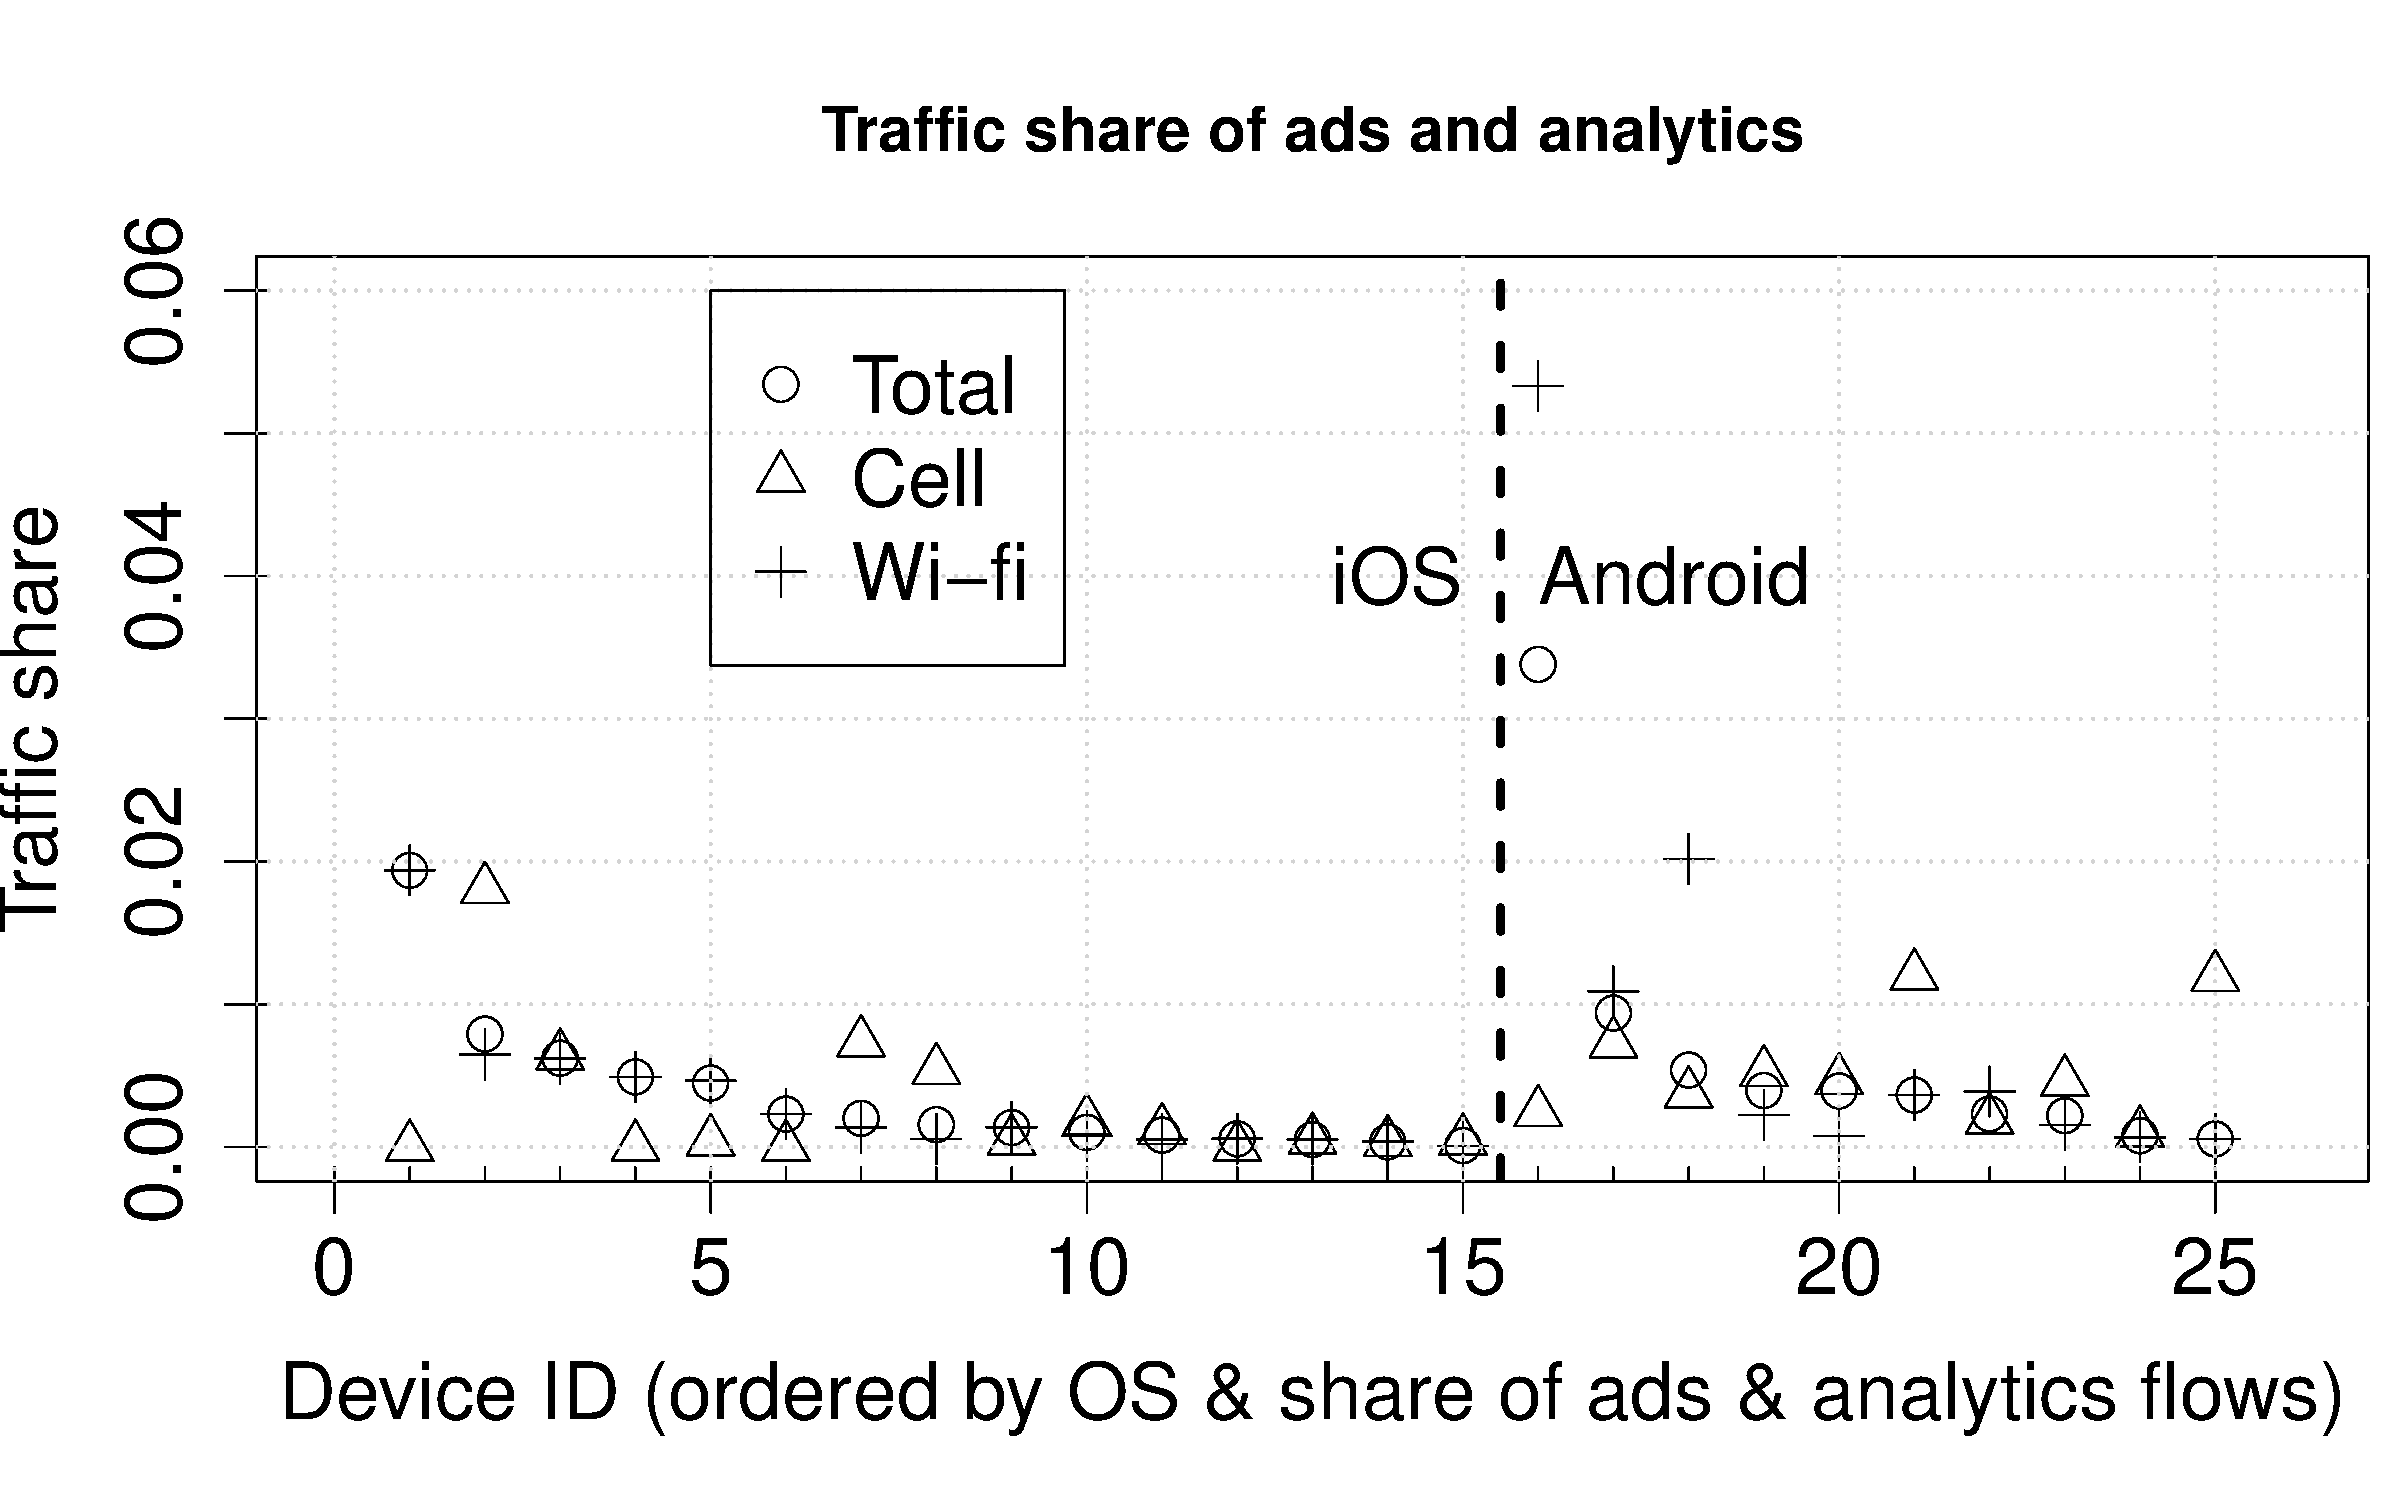
\includegraphics[width=\columnwidth]{plots/ad_share_bytes.pdf}
\caption{Fraction of traffic volume because of Ads and Analytics. \emph{\tbd{Check for id1 and id25}}}
\label{fig:description}
\end{figure}

\begin{figure}[t]
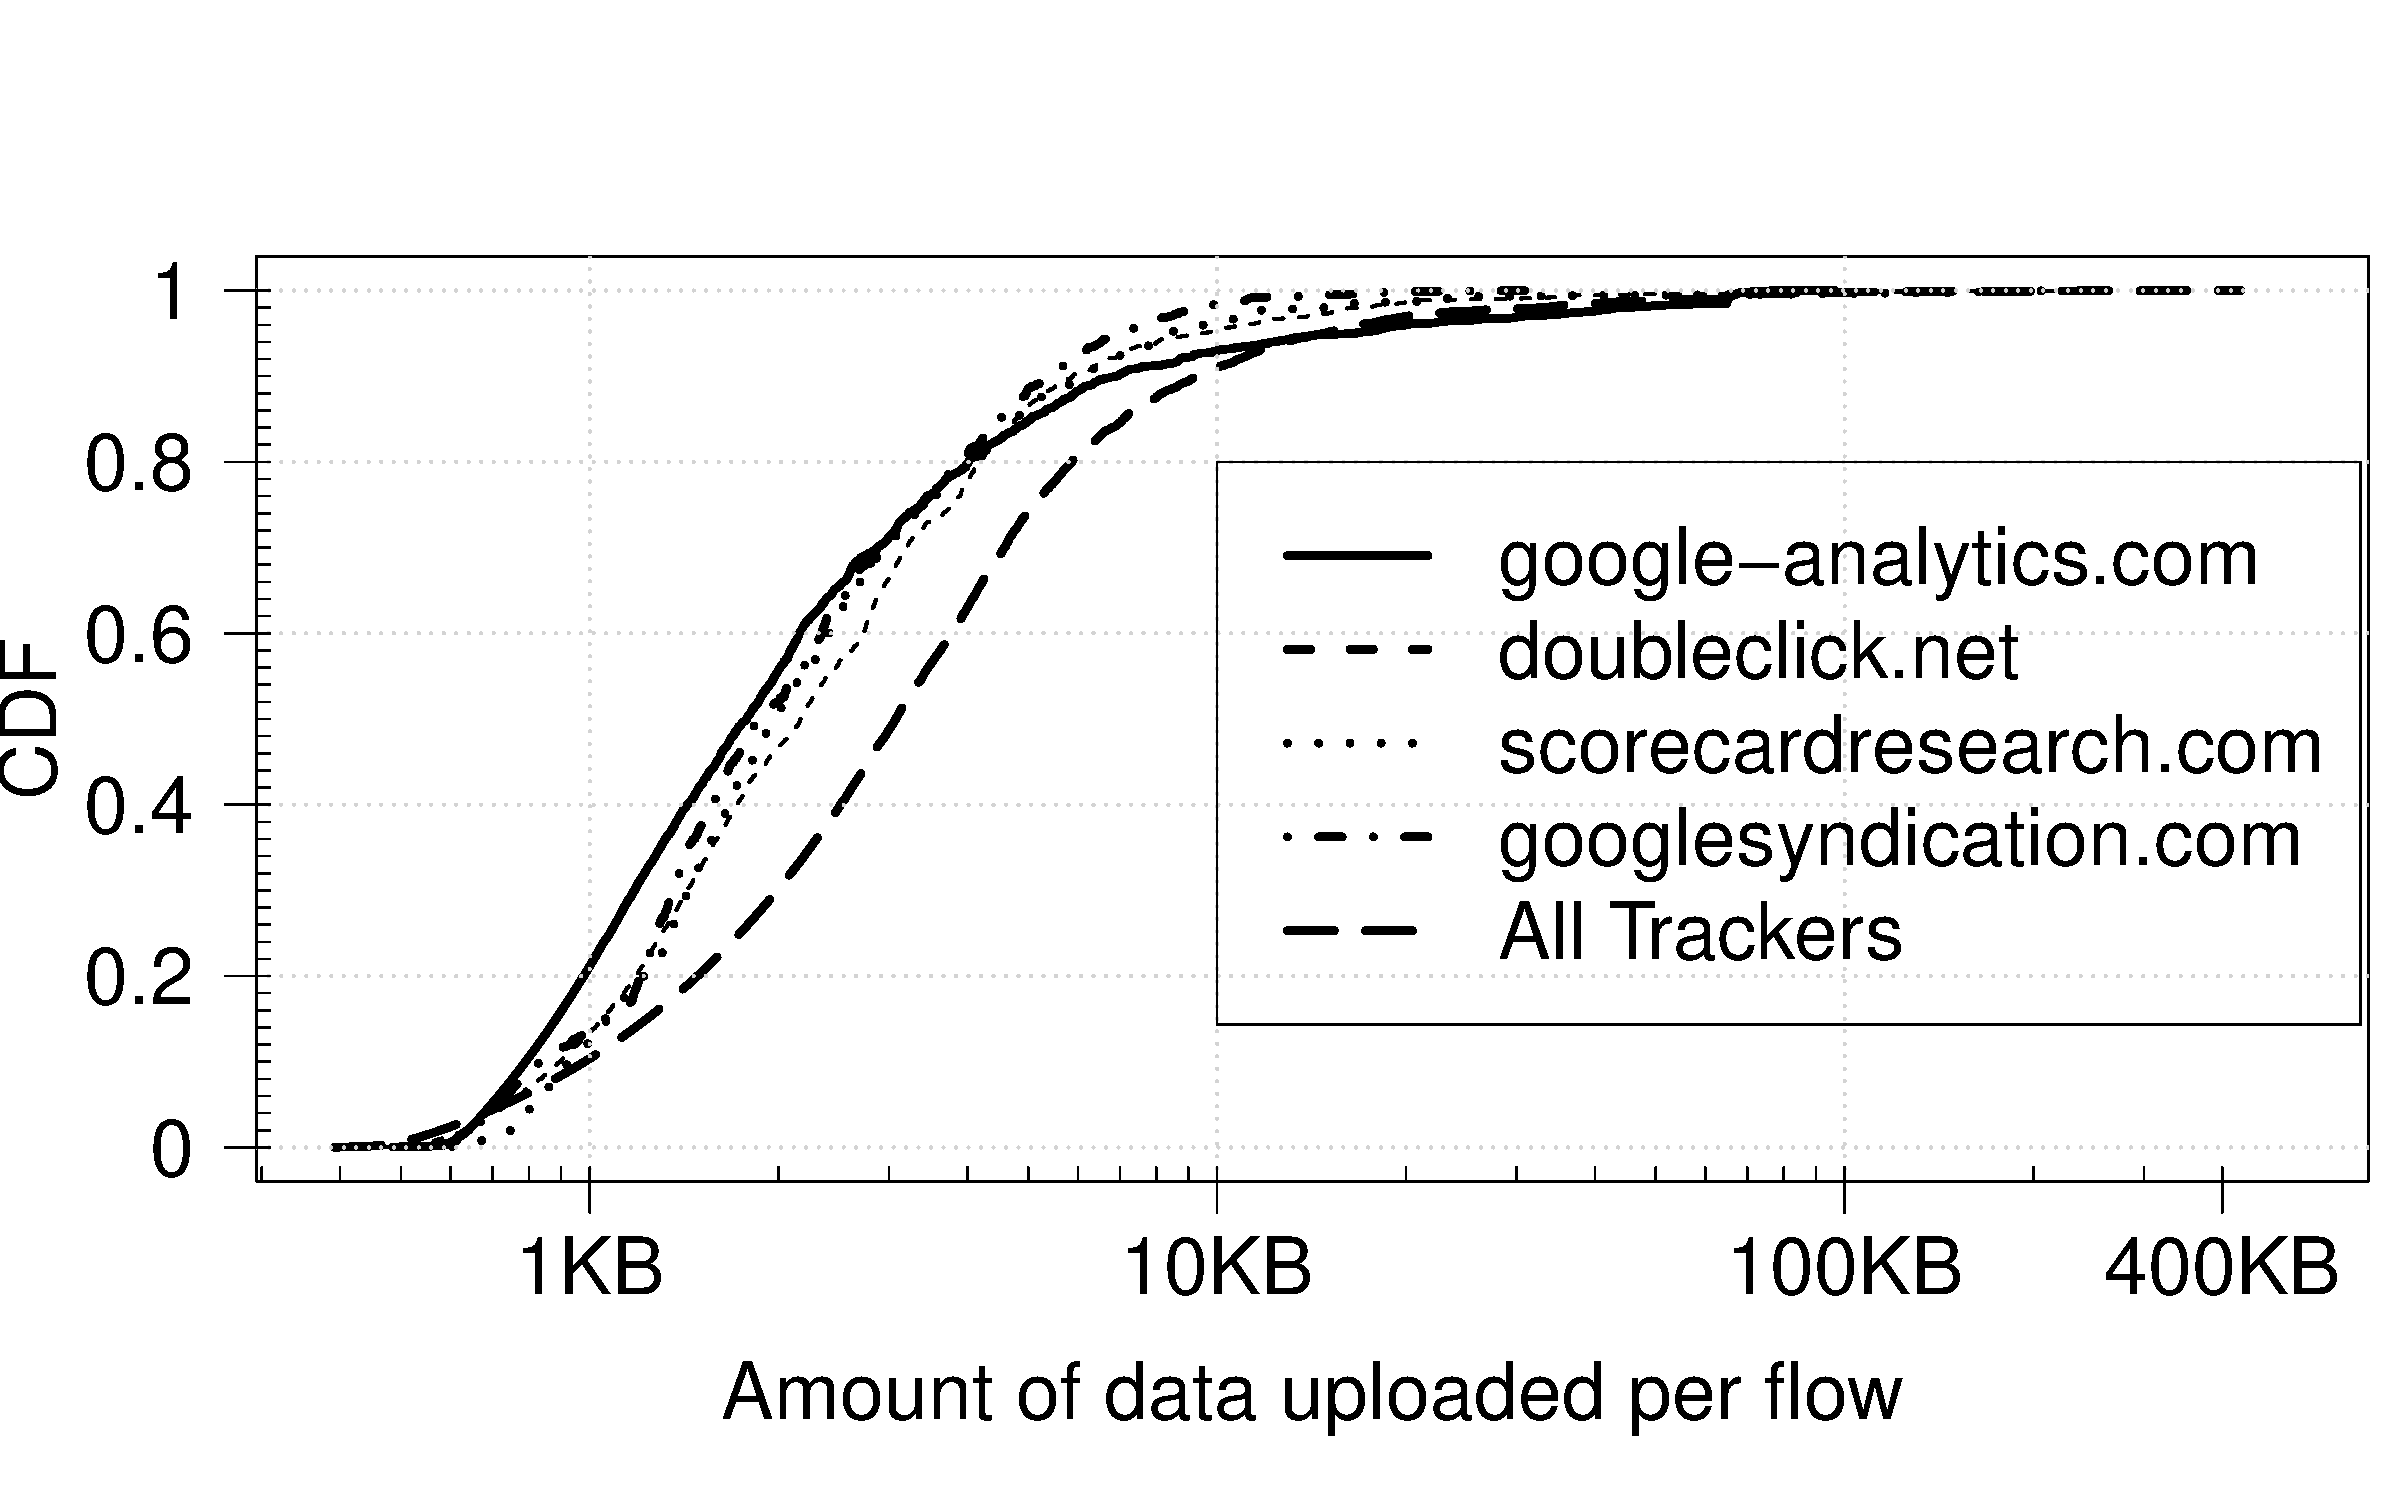
\includegraphics[width=\columnwidth]{plots/distrib_ad_uploads.pdf}
\caption{Distribution of bytes uploaded by ads and analytics sites. \emph{The distribution of bytes uploaded by all ads and analytics sites and the top four ads sites based on traffic volume across all users}.}
\label{fig:description}
\end{figure}

\begin{figure}[t]
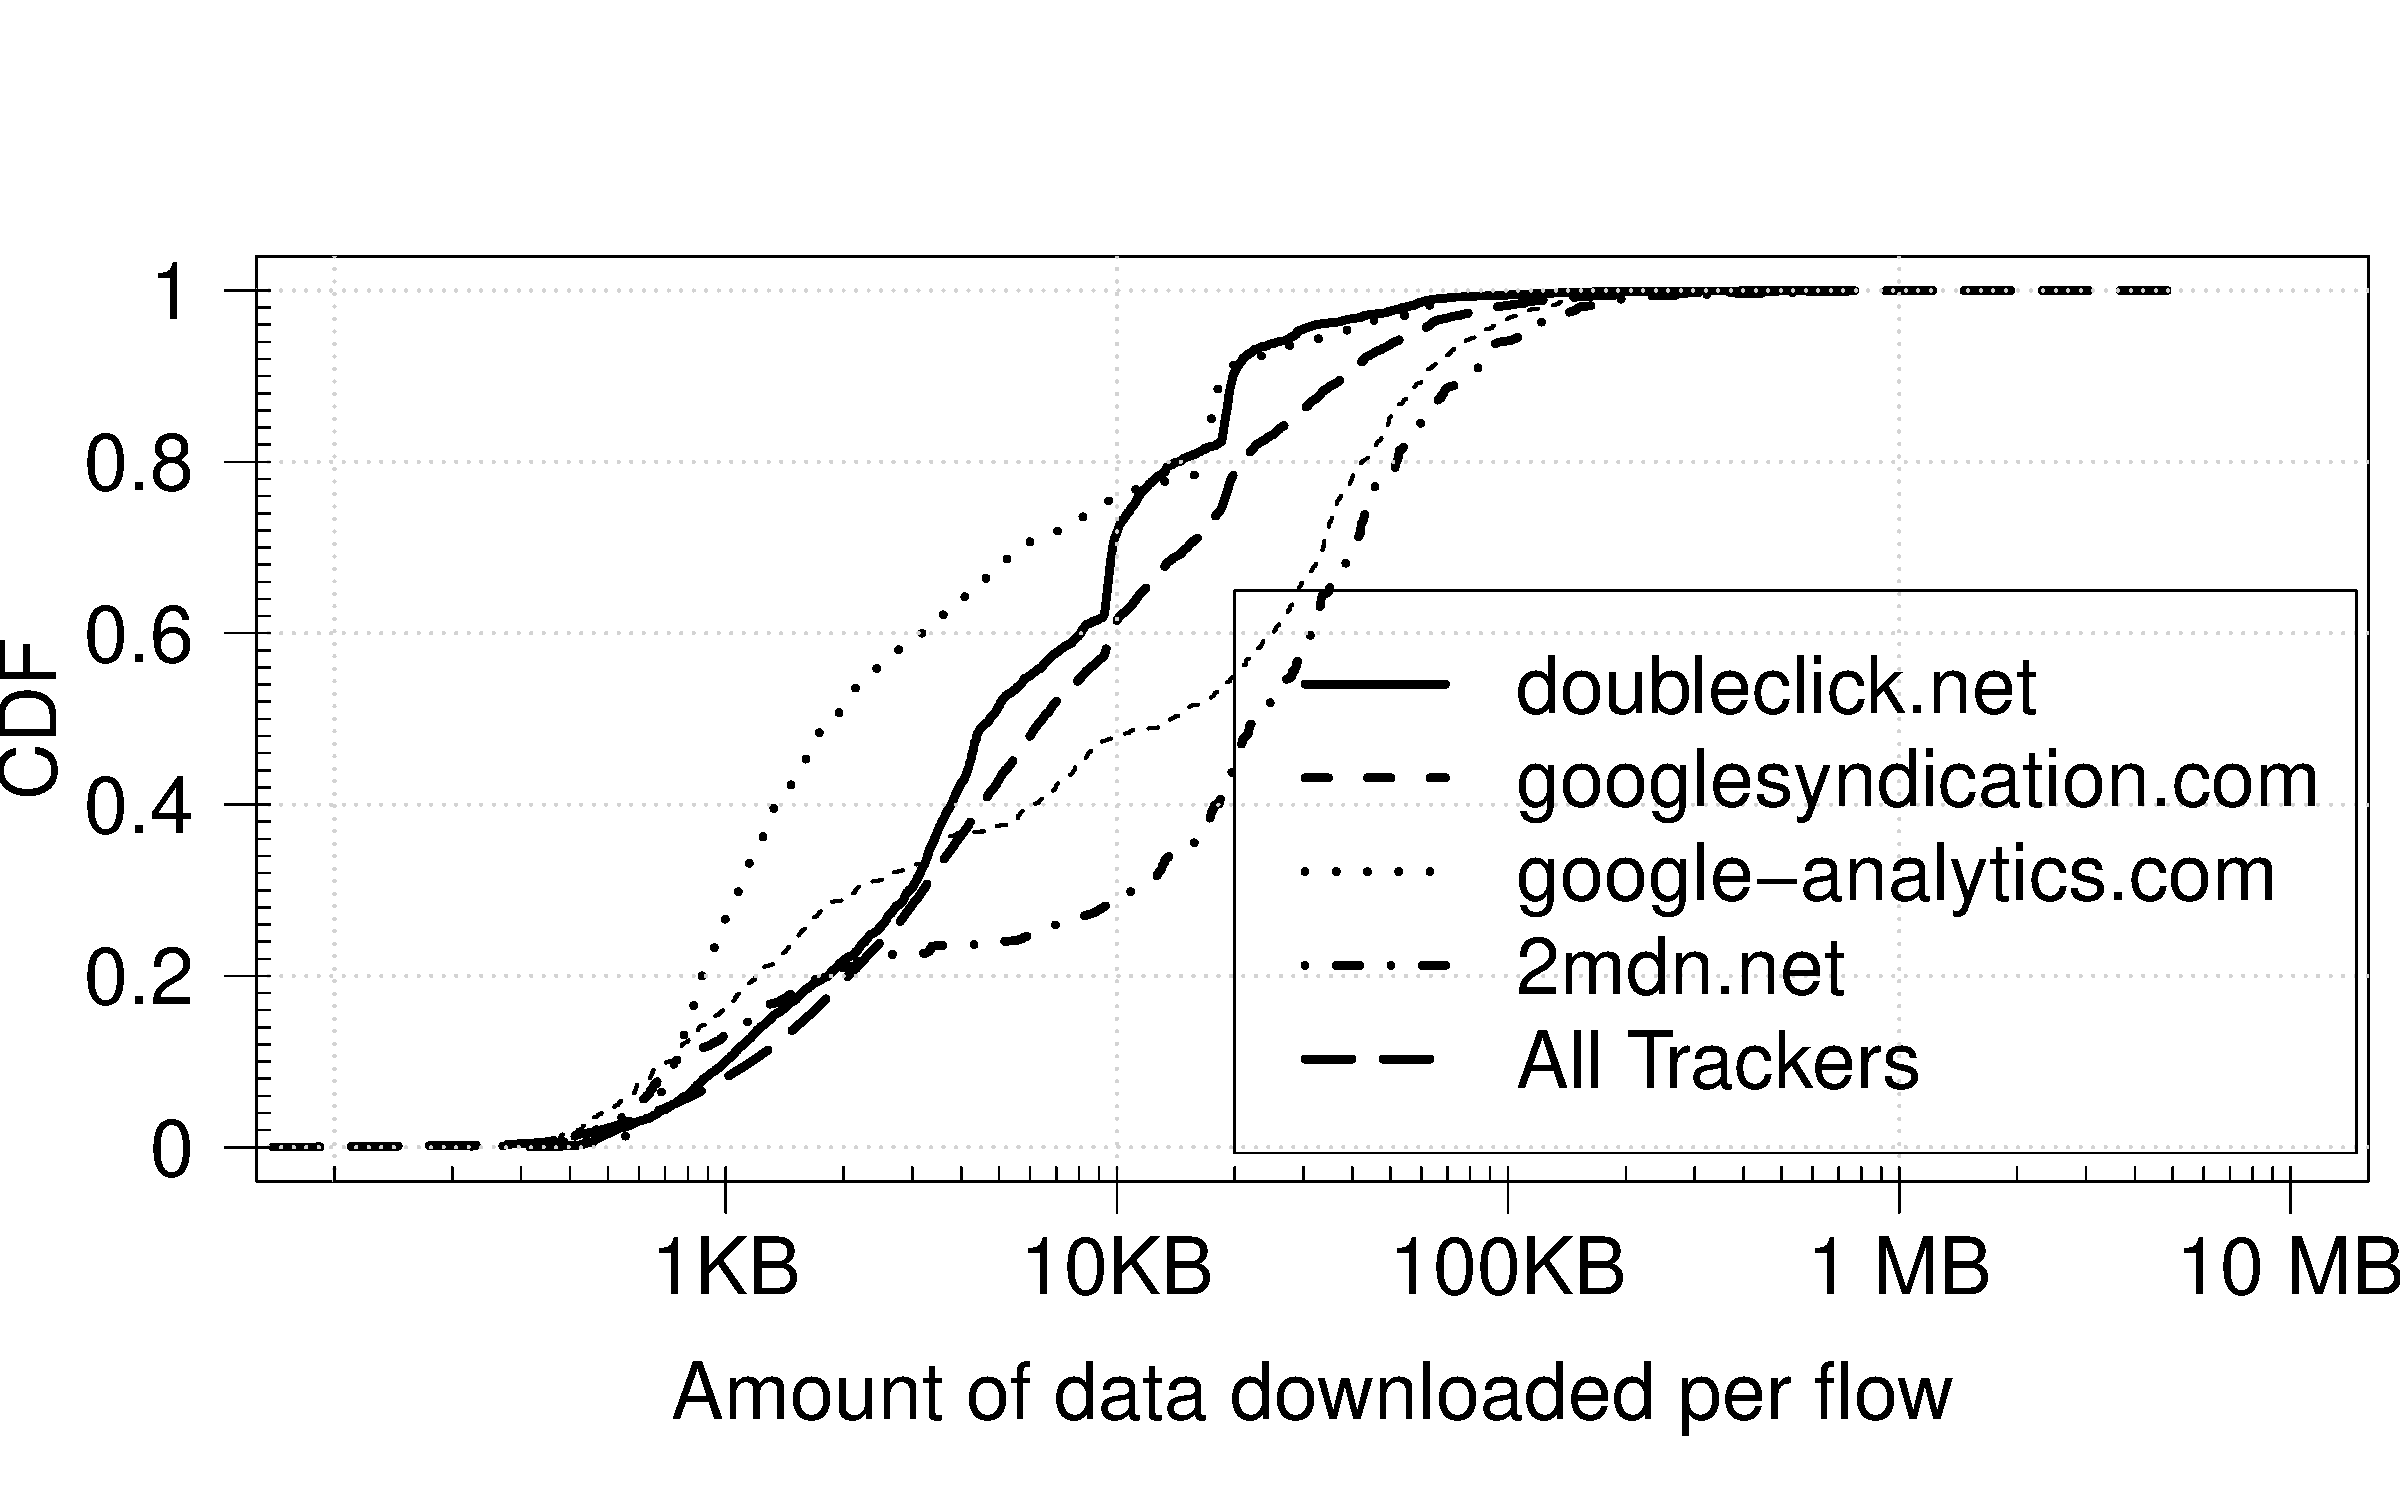
\includegraphics[width=\columnwidth]{plots/distrib_ad_downloads.pdf}
\caption{Distribution of bytes downloaded by ads and analytics sites. \emph{The distribution of bytes uploaded by all ads and analytics sites and the top four ads sites based on traffic volume across all users}.}
\label{fig:description}
\end{figure}

\begin{table}[t]
\centering
\begin{small}
\begin{tabular}{|p{0.35\columnwidth}|p{0.1\columnwidth}|p{0.15\columnwidth}|p{0.1\columnwidth}|}
\hline
\multirow{2}{*}{\bf Tracker} & \multicolumn{3}{c|}{\bf Number of devices tracked}\tabularnewline
\cline{2-4}
   &  {\bf Total} & {\bf Android} & {\bf iOS} \tabularnewline
\hline
doubleclick.net & 25 & 11 & 14 \tabularnewline
\hline
google-analytics.com   & 25 & 11 & 14 \tabularnewline
\hline
googlesyndication.com  & 22 & 10 & 12 \tabularnewline
\hline
admob.com  & 21 & 10 & 11 \tabularnewline
\hline
scorecardresearch.com &  21 & 10 & 11 \tabularnewline
\hline
2mdn.net  &  20 & 9 &  11 \tabularnewline
\hline
atdmt.com  & 18 & 9 &  9 \tabularnewline
\hline
imrworldwide.com & 18 &  9 &  9 \tabularnewline
\hline
flurry.com & 17 & 7 &  10 \tabularnewline
\hline
googleadservices.com  & 17 & 8 &  9 \tabularnewline
\hline
\end{tabular}
\end{small}
\caption{The top 10 ads and analytics sites that tracked the devices in our dataset.
\emph{Two trackers, \emph{doubleclick.net} and\emph{google-analytics.com}, were tracking all the 25 devices in our dataset.}}
\label{tab:top_trackers}
\end{table}


\begin{table*}[t]
    \begin{tabular}{l|l|l|l|l|l|l|l|l|l|l}
       Dataset&Platform&Proto&\# Apps&Email&Location&Username&Password&Android ID&Contacts&IMEI\\
       \hline
       Google Play&Android&HTTP&100&?&10 (10\%)&7 (7\%)&1 (1\%)&21 (21\%)&0 (0\%)&13 (13\%)\\
       \hline
       Third Party&Android&HTTP&908&?&32 (3.5\%)&?&0 (0\%)&95 (10.4\%)&4 (0.4\%)&48 (5.3\%)\\
       \hline
       App Store&iPhone&HTTP&100&?&?&?&?&?&?&?\\
    \end{tabular}
    \caption{\label{tbl:pii}Summary of personally identifiable information leaked in plaintext (HTTP) by Android and iPhone apps.}
  \end{table*}
  

  {\bf Android Apps.}
  When we inspect the data from our controlled study, we see that some apps contact a large number of external servers while others contact significantly fewer.
  In Figure~\ref{fig:android-cdns}, we show both the total number of servers contacted (solid lines) as well as the number of organizations contacted (dotted lines) for both the top-100 Google Play dataset and the top-2000 third-party dataset.
  To quantify ``organizations contacted'', we performed whois lookups on all servers contacted and mapped them to an organization name, allowing us to tighten our upper bound on the number of companies/entities able to track the user through a single app.
  Returning to the figure, we see...~\ref{fig:android-cdns}...\tbd{Amy...}


  {\bf iPhone Apps.}
  \tbd{Shen...}

\subsection{Personally Identifiable Information}
 
  Finally, we turn to information leaked by individual applications. We do not report on data leaked for our real users here, but only the data leaked by our controlled apps in isolation.
  We created fake user accounts on the test phones for a fake user named ``Tess Droid'', with fake contact information and fake Twitter and Facebook accounts. 
  We were then able to check that none of this data ever was released over the network, either in plaintext (HTTP) or encrypted (HTTPS, see \S\ref{sec:bumping}).
  
  We consider data to be `leaked' when any personally identifiable information -- email address, phone number, IMEI number -- is sent across the network under HTTP or HTTPS.
  Some of this information may be relevant to the app -- \eg{}, many apps legitimately require email access. 
  However, none of this information should ever travel across the network in plaintext (HTTP), which we see violated in serveral cases.

  In Table~\ref{tbl:pii}, we see the type of PII leaked for both Android and iPhone apps.
  For Android apps, IMEI and Android ID are the most commonly leaked forms of PII in both the Google Play and third-party dataset.
  Although not popularly thought of as ``private'' data, each of these identifiers are globally unique: IMEI is a unique identifier tied to a phone, and an Android ID is an identifier tied to a user's Google Account, used across many services on the Internet. 
  Consequently, either of these datapoints can be used to track or correlate a user's behavior across all sites the user visits that sell or collaborate with tracking data: a user's behavior on one site can easily be linked to their behavior on any other site they visit.
  With Android ID being tracked by between 10 and 20\% of apps in our study, and IMEI being tracked by between 5\% and 13\% of apps in our study, this suggests that global user tracking across collaborating services can be easily achieved today just by using this identifier.
  \tbd{...}

  Other informaiton like contacts, email, and passwords were rarely leaked in the clear, but all were leaked on occaision, suggesting that stricter monitoring of Android app behavior is needed -- contrastingly, no iPhone apps (which are manually given clearance by Apple before hitting the iPhone store) leaked passwords in plaintext~\tbd{is this true.}

  Moving to iPhone apps, \tbd{...}
%\subsection{Characterize Facebook Applications}

%Why Facebook was chosen?

%What do we observe ?

%What do we see in the User Agent Fields. 




\section{Behavior of Networks}

\subsubsection{Controlled Experiments}

\subsubsection{In the Wild}

We ignore connections from the same network and ISP in which our servers were placed.


\begin{figure}[t]
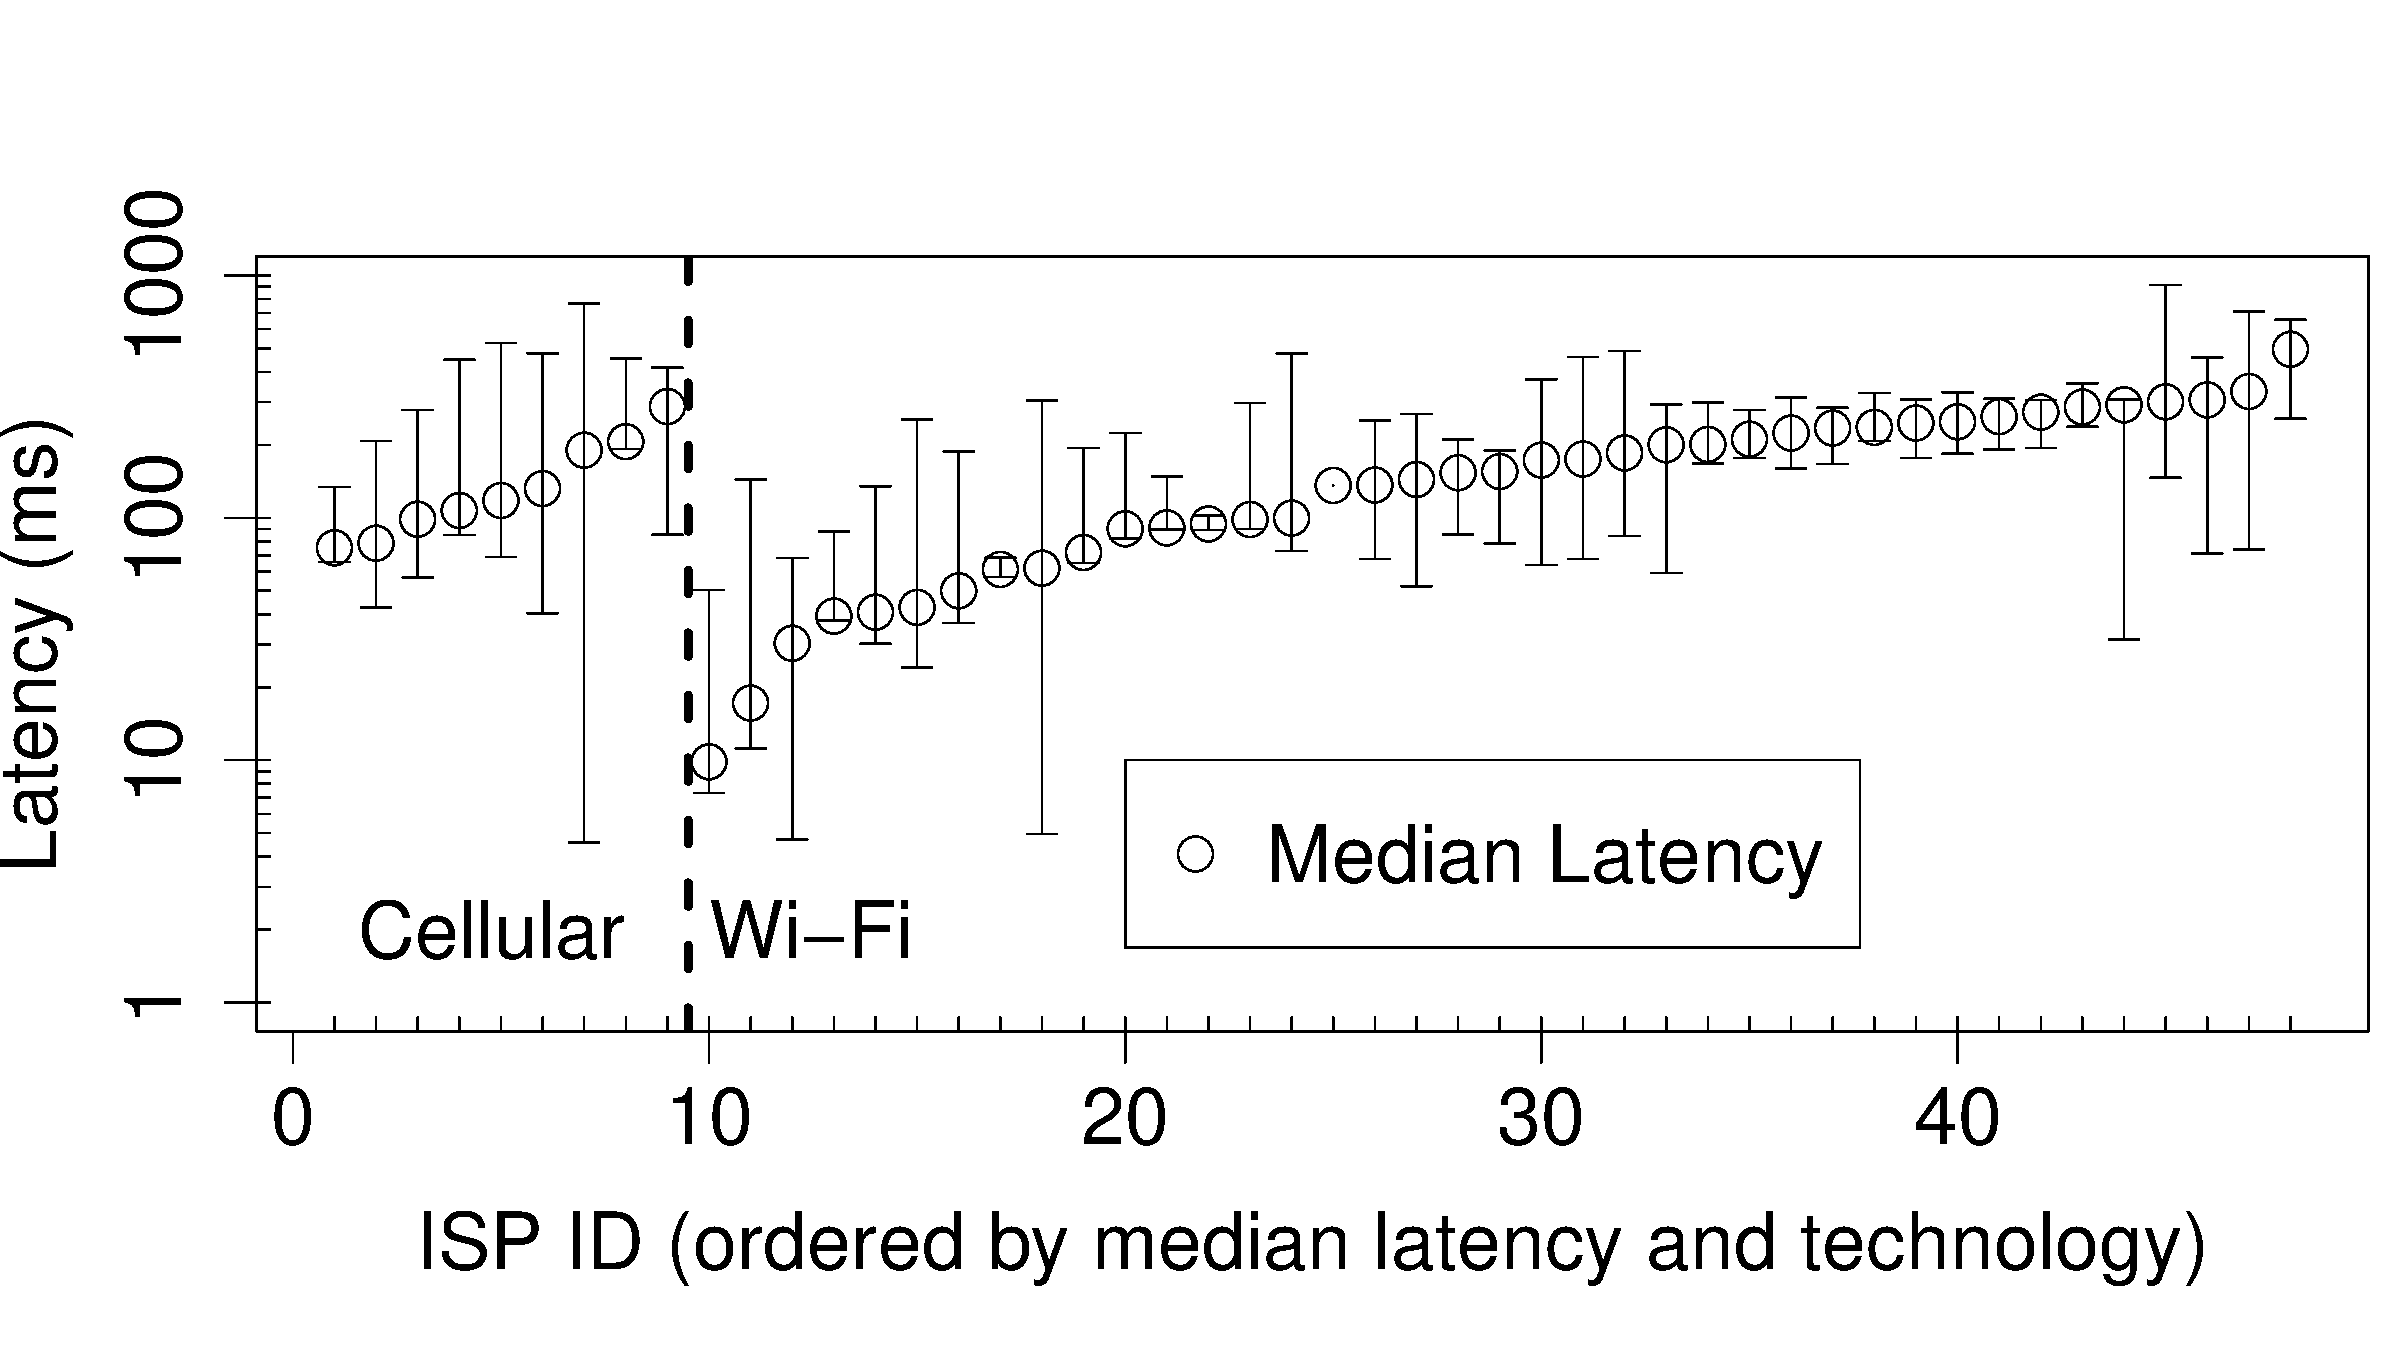
\includegraphics[width=\columnwidth]{plots/latency_isp_whisker.pdf}
\caption{One-way latency from VPN server to mobile devices. \emph{Connections from cellular ISPs suffer a higher delay compared to Wi-Fi ISPs. The delays from Cellular ISPs is comparable to connecting from a Wi-Fi ISP in another country. Error bars indicate the 91st and 9th percentile}.}
\label{fig:latency-across-isps}
\end{figure}


\begin{figure}[t]
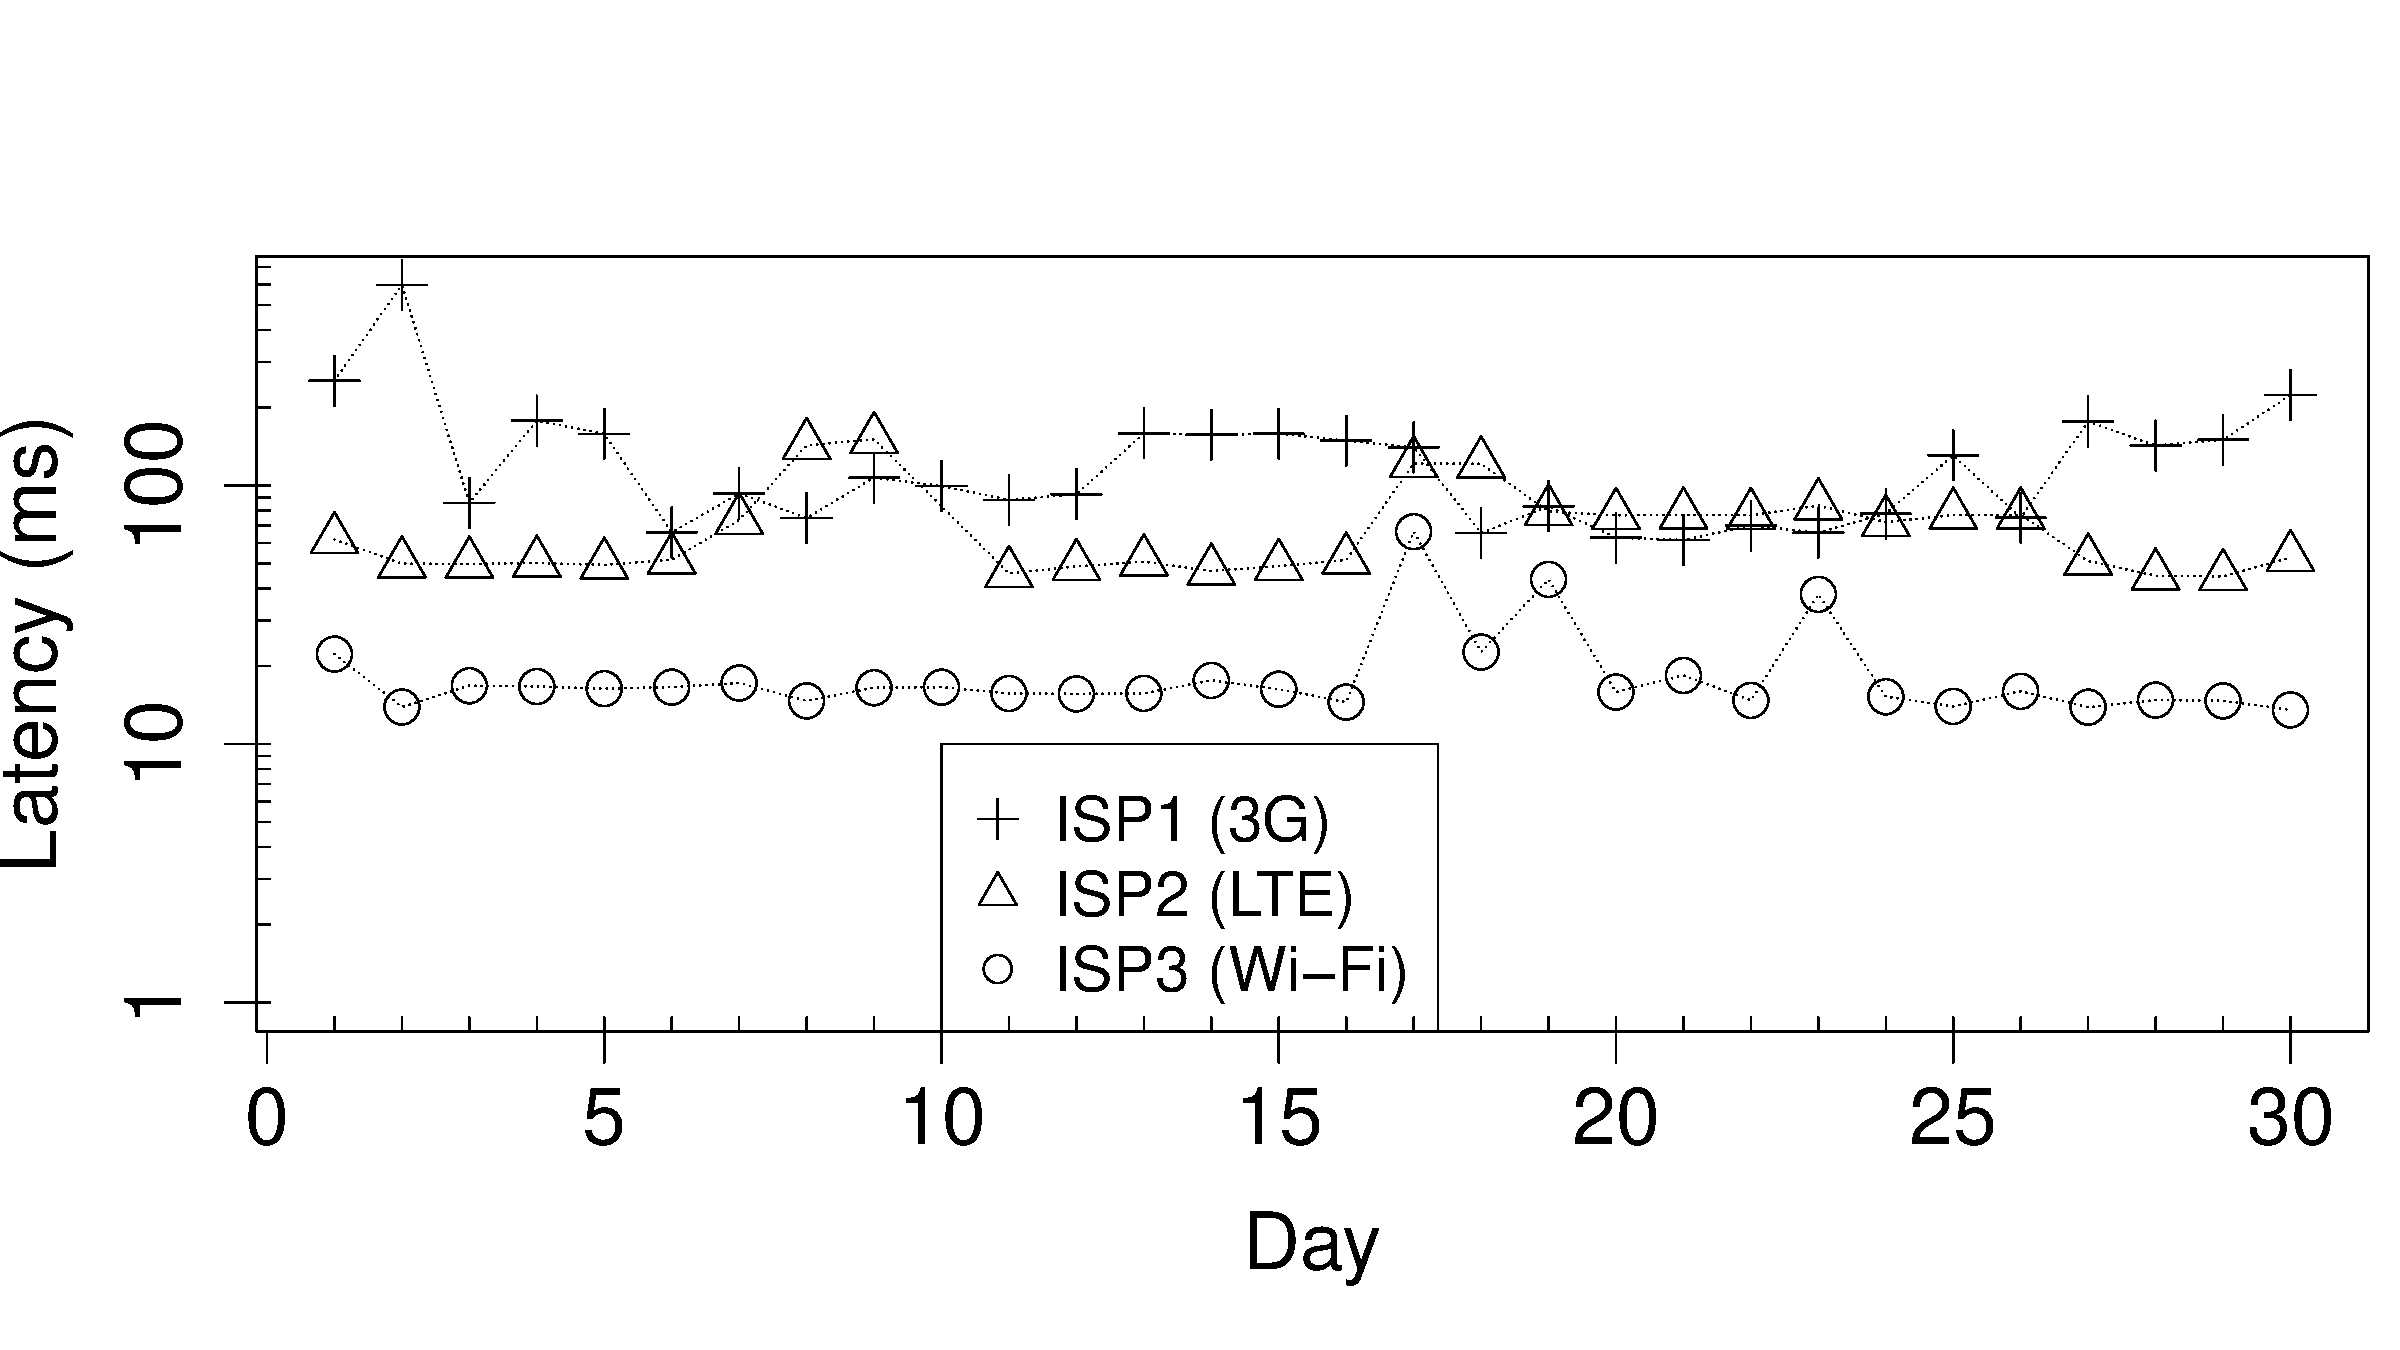
\includegraphics[width=\columnwidth]{plots/compare_isp_latency.pdf}
\caption{Comparison of ISPs that serve the same user during a 30 day time period. \emph{The LTE service provider has a smaller latency to the 3G provider. The smallest latency is observed by in the home Wi-Fi network.}}
\label{fig:compare-isp-latency}
\end{figure}

\begin{figure}[t]
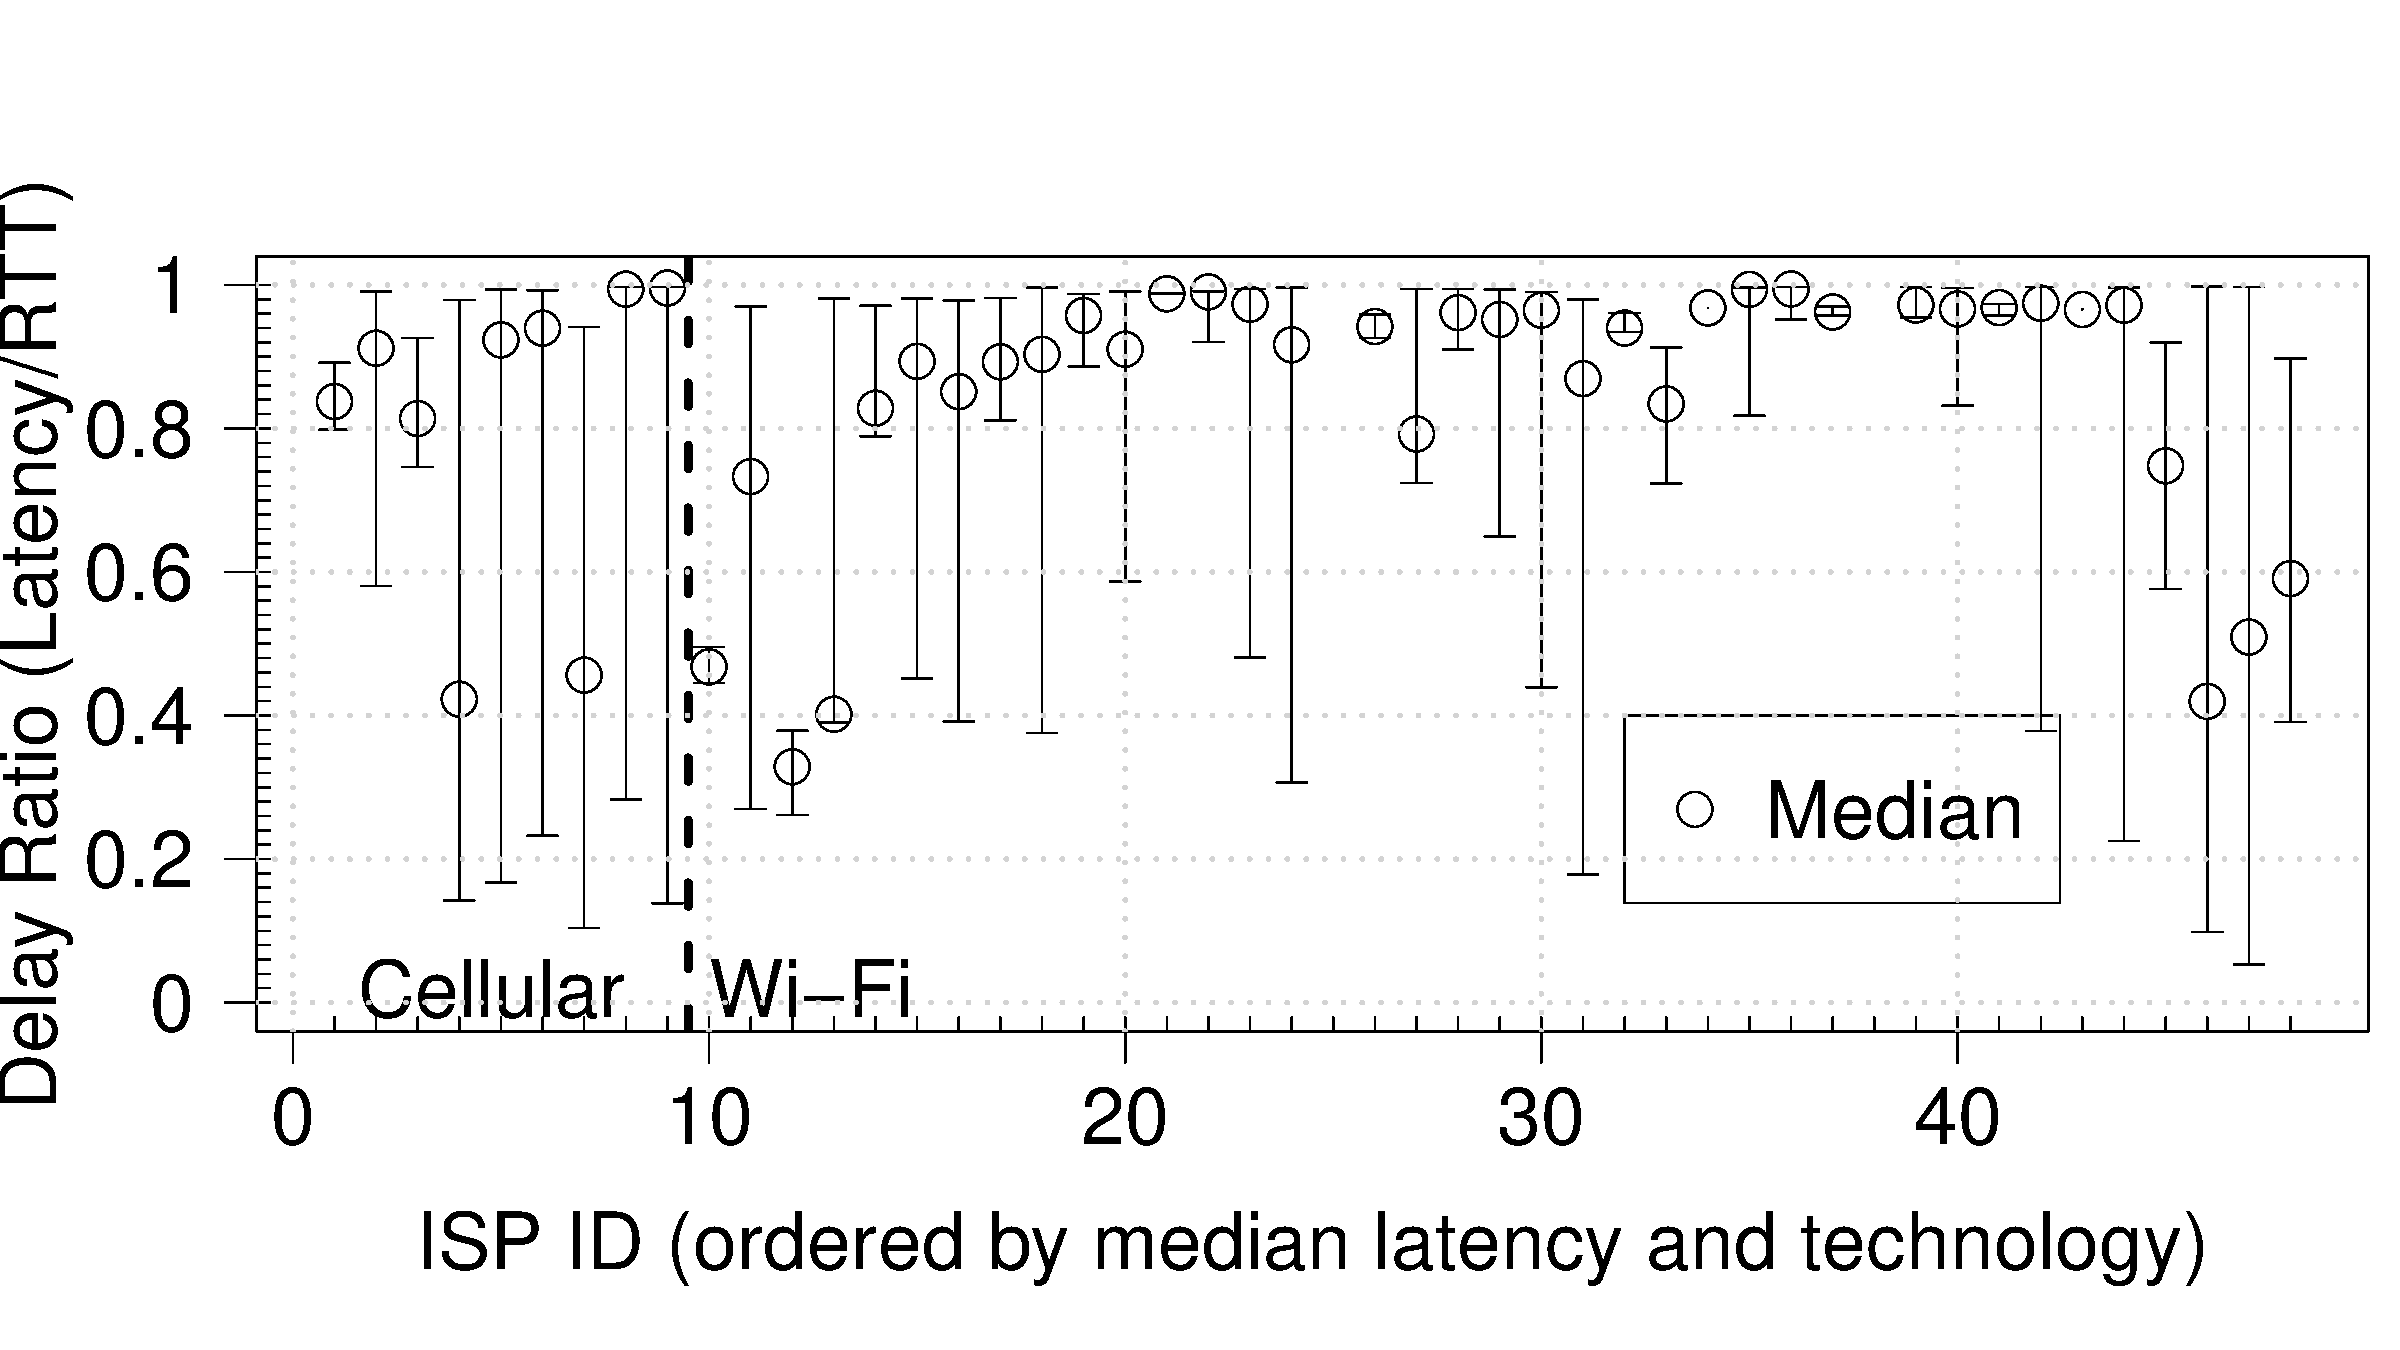
\includegraphics[width=\columnwidth]{plots/delay_ratio_isp_whisker.pdf}
\caption{Latency as a fraction of the round trip time to contact google services. \emph{In 35 ISPs of the 48 ISPs we observe that the latency of the mobile device to our server accounts for more than 90\% of the end-to-end round trip time. Error bars indicate the 91st and 9th percentile.}}
\label{fig:compare-delay-ratio}
\end{figure}

\begin{figure}[t]
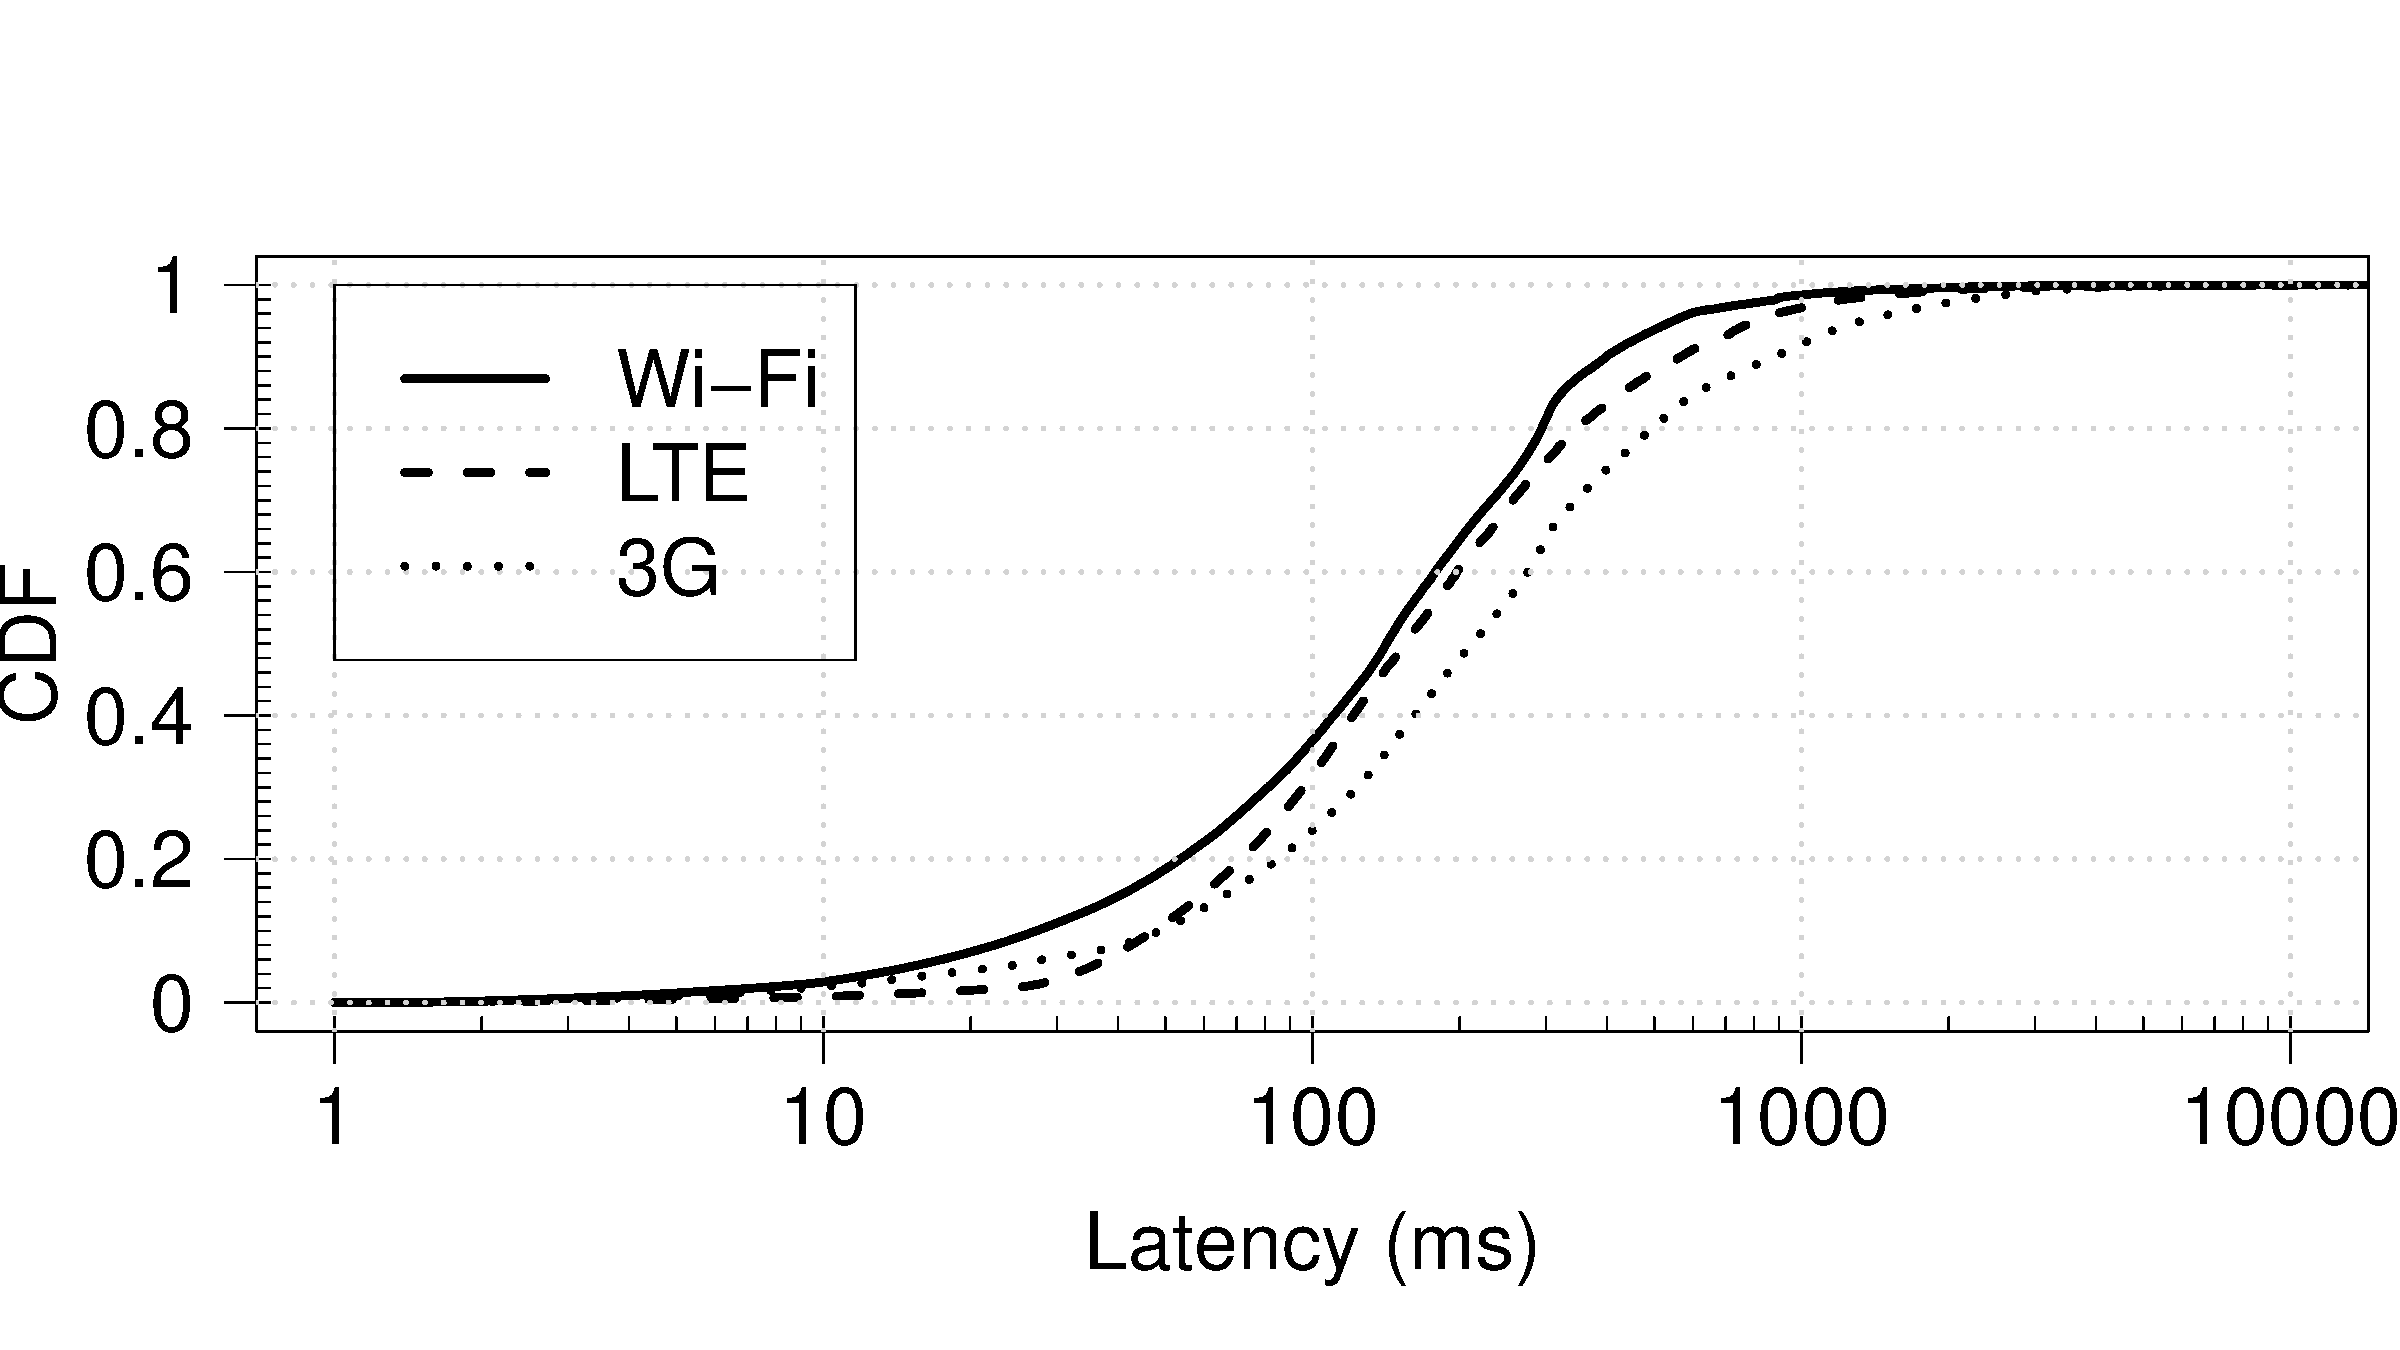
\includegraphics[width=\columnwidth]{plots/distrib_latency_technology.pdf}
\caption{Distribution of latency over cellular and \wifi ISPs. \emph{The distribution of latency observed when using LTE in the wild is similar to that observed for \wifi}.}
\label{fig:compare-delay-ratio}
\end{figure}

\begin{figure}[t]
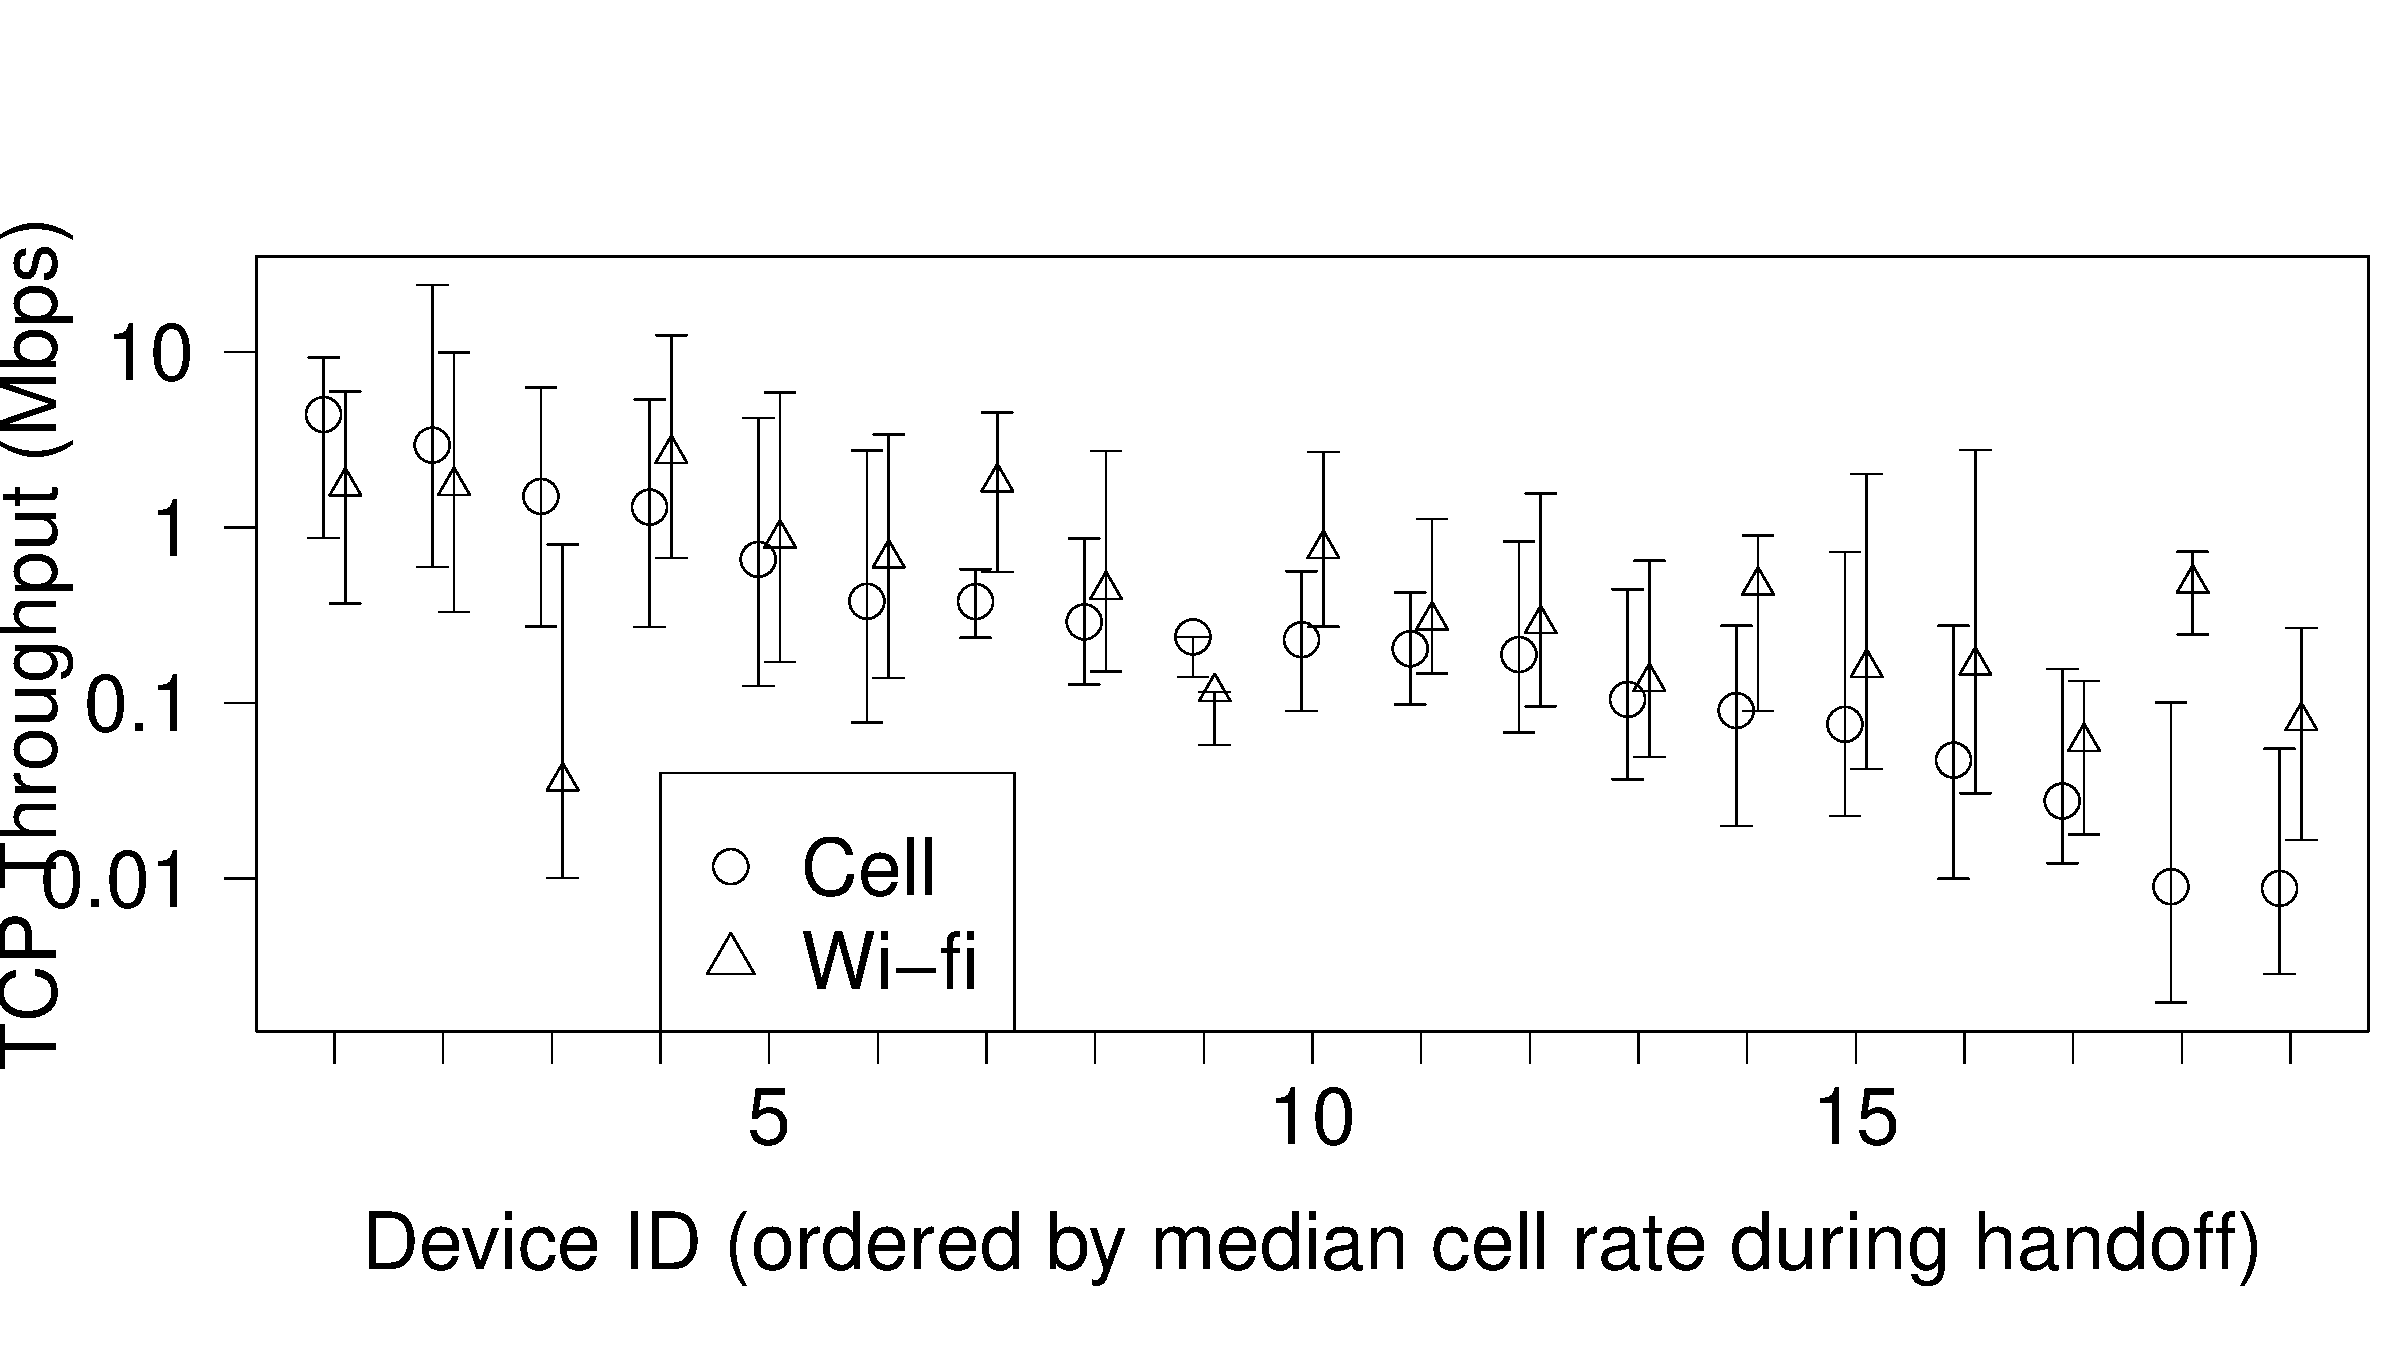
\includegraphics[width=\columnwidth]{plots/handoff_rates.pdf}
\caption{TCP Throughput observed during the hour of the handoff. \emph{The three users that have LTE connections observed a better TCP throughput over LTE in comparison to \wifi in the hour of the handoff. Error bars indicate the 91st and 9th percentile}.}
\label{fig:compare-handoff}
\end{figure}




\tbd{We performed a traceroute from our server to the egress link and found }





\section{Related Work}
\label{sec:related}

The network behavior of mobile systems has implications for battery life, 
data-plan consumption, privacy, security and performance, among others. 
When attempting to characterize this behavior, researchers face a number 
of trade-offs: compromising network coverage (limiting the number and type of ISPs measured), 
portability (limiting the device OSes) and/or deployability (limiting subscriber coverage).
\platname compromises 
none of these, enabling comprehensive measurements across carriers, devices and access 
technologies. Table~\ref{tab:relatedCompare} puts our approach in context with previous 
approaches for measuring the network behavior of mobile systems. 

\begin{table*}[t]
\begin{center}
{\footnotesize
\begin{tabular}{|l|l|l|l|l|}
\hline
 & \textbf{Network Coverage} &  \textbf{Portability} &  \textbf{Deployment model} &   \textbf{Meas. Type}  \\ \hline
AT\&T/Telefonica study~\cite{vallina-rod:ads,gerber:passivespeed} & Single carrier & All OSes & Instrument cell infrastructure & Passive \\ \hline
WiFi study~\cite{chen:wifi} & Single WiFi network & All OSes & Instrument WiFi network & Passive \\ \hline
PhoneLab/TaintDroid~\cite{enck:taintdroid} & Multiple networks & Android & Install custom OS & Active/Passive \\ \hline
MobiPerf~\cite{wang:middleboxes}/SpeedTest~\cite{sommers:cellwifi} & Multiple networks & Android & Install App & Active \\ \hline
\platname & Any network & Android / iOS & VPN configuration & Passive \\ \hline
\end{tabular} }
\end{center}
\label{tab:relatedCompare}
\caption{Comparison of alternative measurement approaches. \platname is the first approach to cover all access networks and most device OSes, capturing 
network traffic passively and with low overhead via VPN proxying.}
\end{table*}%

Traces from mobile devices can inform a number of interesting analyses. Previous work 
uses custom OSes to investigate how devices waste energy~\cite{pathak:eprof}, network bandwidth and 
leak private information~\cite{enck:taintdroid,hornyack:appfence}. Similarly, AppInsight~\cite{ravindranath:appinsight} and PiOS~\cite{egele:pios} can inform 
app performance through binary instrumentation and/or static analysis. In this work, we explore the opportunity to use network traces 
alone to reveal these cases without requiring any OS or app modifications.

Network traces from inside carrier networks provide a detailed view for large numbers 
of subscribes. For example, Vallina-Rodriguez~\etal~\cite{vallina-rod:ads} uses this approach to characterize performance and 
the impact of advertising. Gerber \etal~\cite{gerber:passivespeed} similarly use this approach to 
estimate network performance for mobile devices.  \cite{maier:mobtraffic} \cite{chen:wifi}
Similar to these approaches, \platname provides continuous passive monitoring of mobile network 
traffic; however, \platname is the first to do so across all networks to which a device connects.

Last, active measurements~\cite{wang:middleboxes,sommers:cellwifi} allow researchers to understand network topologies and instantaneous 
performance at the cost of additional, synthetic traffic for probing. In contrast, \platname uses 
passive measurements to characterize the traffic that devices
naturally generate.

%%% Local Variables: 
%%% mode: latex
%%% TeX-master: "main.tex"
%%% End: 


Bro port based classification of HTTP, SSL, other, and so on. 


\section{Classification of Application}

\platname enables us to monitor the data being exchanged by the mobile device. 
However, it does not provide any details of the source of the data. 
We use the following technique to estimate the source of the mobile data traffic. 
In \ref{tab:summaryIOSAndroidTraffic} and \ref{tab:summaryWifiCellularTraffic} we observe that TCP is responsible for the majority of the traffic volume from iOS and Android devices regardless of the access technology used. 
We therefore focus on associating TCP flows to the applications for our analysis. 
From our analysis we were able to classify \tbdv{x\%} of the TCP traffic volume and \tbdv{y\%} of the TCP flows to the applications.

\subsection{Methodology}

\subsection{Results}

User Agent based classification
flows per user with a blank user agent. 
flows per user with a default user agent 
flows with application in user agent


SSL certificate based classification
flows to dedicated hosts
flows to cdns

\subsection{Discussion}

\section{Specific application behavior}


\section{Ads and Analytics}

Ads and Analytic sites have received considerable attention.
The reason for the attention being the intrusiveness exhibited by the ads and analytics sites in tracking personal information. 
\cite{vallina-rod:ads} show that \tbdv{ } of data traffic volume observed from a Cellular ISP is because of mobile ads. 
In our traces we use the classification of \cite{vallina-rod:ads} and \cite{YoyoAds} to classify flows as ads flows. 



\section{Discussion on Platform}

IPv6 support of VPNs

ISP support of VPNs. One ISP blocked VPN access. 

Open source ??

Releasing datasets ??


